\section{Introduction}

The addition of microstructure control in bijels can be utilized to improve the performance of porous materials
or soft matter derived from their co-continuous, tortuous microstructure. The importance of microstructure control
allows an increase in the charge/discharge rate of batteries through reducing the material tortuosity, or improving the 
adhesion and growth rate of bone grafts. These properties are imparted during the fabrication step of the bijel. Anisotropic
particles adsorbed at interfaces induce shape-dependent capillary interactions that have distinct effects on the
microstructure of emulsions, resulting in migration or rotation of particles at interfaces, in addition to the addition of
distinct timescales of domain coarsening. \cite{loudet_capillary_2005, cavallaro_curvature-driven_2011, gunther_lattice_2013}

In bijels, ellipsoidal stabilizers have been demonstrates to result in additional timescales of domain coarsening 
at long timescales owing to particle re-orientation at the interface due to interparticle capillary interactions 
at long timescales. \cite{gunther_timescales_2014} In addition to possessing more timescales, property, bijels stabilized 
with rod-like particles have been shown to result in smaller characteristic length scales, owing to the particles having a
larger cross sectional area resulting in jamming occurring at larger interfacial areas. \cite{hijnen_bijels_2015} 

Magnetic response has been used in particle stabilized emulsions in the past, causing controlled emulsion failure and
on-demand droplet coalescence for encapsulation and cargo release applications. \cite{melle_pickering_2005, zhou_magnetic_2011}
Fields also enable self assembly through the control of interface deformation derived capillary forces.
\cite{morgan_understanding_2013,davies_interface_2014,davies_dipolar_2015} Magnetically responsive spherical particle 
stabilized bijels have thus far not yielded significant microstructural modifications. \cite{kim_bijels_2010} However, 
electric fields have been shown to cause percolating cylindrical domains in electrically responsive bijels. \cite{carmack_tuning_2018}
The electric field causes polar interactions between particles, which causes the formation of chains of particles that
also function as nucleation sites for phase separation. \cite{carmack_tuning_2018}

In this chapter, we investigate the effect of external magnetic fields on the formation of bijels stabilized by 
anisotropic magnetic particles. The microstructure of bijels stabilized with oblate, spherical and prolate particles, 
namely the characteristic length scale and tortuosity, will be assessed as a function of the applied magnetic field
strength. We also characterize the underlying mechanisms governing the observed behavior. 

% Anisotropic particles, when adsorbed at liquid interfaces, induce
% shape-dependent capillary interactions that can have a distinct effect
% on the microstructure of emulsions
% \cite{loudet_capillary_2005,loudet_self-assembled_2009}. For instance,
% Madivala et
% al.~\cite{madivala_exploiting_2009,madivala_self-assembly_2009} found
% that emulsion stability can be significantly enhanced by ellipsoidal
% particles. Additionally, capillary interactions can lead to direct
% assembly of anisotropic particles
% \cite{bowden_self-assembly_1997,lewandowski_orientation_2010,stebe_oriented_2009,botto_capillary_2012}.
% Ellipsoidal particles can rotate and migrate on curved surfaces
% \cite{cavallaro_curvature-driven_2011}, where the interface curvature
% acts as an external field that controls the orientation and placement
% of particles \cite{furst_directing_2011}. Anisotropic particles at
% fluid interfaces were considered in Monte Carlo simulations by Bresme
% et al. to test the accuracy of thermodynamic models for the free
% energy as a function of the particle-fluid interactions, particle
% size, and orientation
% \cite{bresme_orientational_2007,bresme_computer_2008}. Harting and
% co-workers \cite{gunther_lattice_2013,gunther_timescales_2014} have
% performed lattice Boltzmann simulations of anisotropic particles at
% liquid interfaces and in emulsions. They found that anisotropic
% particles affect the dynamics of emulsion formation by introducing two
% additional timescales associated with particle rotation. Following
% initial adsorption, particles rotate to align their larger
% cross-section with the interface. When jamming sets in, capillary
% interactions cause the particle to re-orient in the interface leading
% to prolonged coarsening at long timescales. Due to the larger aspect
% ratio, ellipsoidal particles can stabilize a larger interface area
% leading to smaller domain sizes. Hijnen et
% al.~\cite{hijnen_bijels_2015} experimentally realized bijels
% stabilized by colloidal rods and analyzed their effect on the
% interface and domain morphology. Their experiments confirmed that
% jamming occurs at lower interface separations than for spherical
% particles with the same volume fraction. Moreover, they observed that
% the overall structure remains isotropic and attributed this to the
% rapid jamming of the rods. Additionally, they found that some rods
% tilted out of the interface due to the compression induced by domain
% coarsening.

% Particle-stabilized emulsions can be made responsive to external
% magnetic fields by magnetic particles
% \cite{melle_pickering_2005,zhou_magnetic_2011}. An external field can
% then be used to control the stability of the emulsion
% \cite{melle_pickering_2005} and the self-assembly of particles
% \cite{dassanayake_structure_2000,leunissen_directing_2009}. The tendency
% of anisotropic particles to adopt distinct orientations gives rise to an
% orientation transition when an external field is applied
% \cite{morgan_understanding_2012,davies_interface_2014,davies_dipolar_2015}.
% Magnetic fields thus offer a means to control the capillary interactions
% of ellipsoidal particles at an interface. For bijels stabilized by
% spherical magnetic particles, simulations by Kim et
% al.~\cite{kim_bijels_2010} revealed that magnetic fields do not have a
% significant effect on the microstructure of bijels. In contrast, Carmack
% and Millett \cite{carmack_tuning_2018} demonstrated that the structure
% of thin-film bijels stabilized by dielectric particles can change
% drastically when an external electric field is applied. The dielectric
% contrast of the particles induces polar interactions that cause liquid
% domain alignment leading to percolating cylindrical domains in the
% thin-film bijel. In addition, they found that particle chains can act as
% nucleation sites for phase separation. This suggests that anisotropic
% interactions can have a considerable effect on the phase separation and
% the resulting emulsion morphology and may offer a means to control the
% size and shape of liquid domains.

\section{Results}\label{sec:results_p1}

Bijels can be used as emulsion templates for porous materials with
applications including drug delivery, water desalination, and battery
electrodes
\cite{vanoli_bijels_2022, chen_pore-scale_2022, lu_controllable_2020, garcia_scalable_2019}.
The transport properties of porous materials depend on the porosity and
tortuosity of the void space and can be linked to the phase-separated
morphology of the bijel template. Therefore, we study the domain size
and tortuosity of the phase morphology of bijels stabilized by
anisotropic particles. In particular, we investigate the effect of
magnetic particles on the microstructure of bijels that are formed in
external magnetic fields. We simulated bijels with a particle volume
fraction of \(\phi_p=0.15\) and varied the magnetic flux density such
that the Bond numbers varies in the range \(0\le\bar{B}\le1\).
In this work, we use a fixed particle volume fraction and focus on the dependence of the 
bijel structure on the magnetic field. Bijels with varying particle loading and surface tension 
and have been studied elsewhere in the literature, e.g., by Hijnen et al.\cite{hijnen_bijels_2015} 
and Jansen and Harting\cite{jansen_bijels_2011}.

\begin{figure}
    \centering
    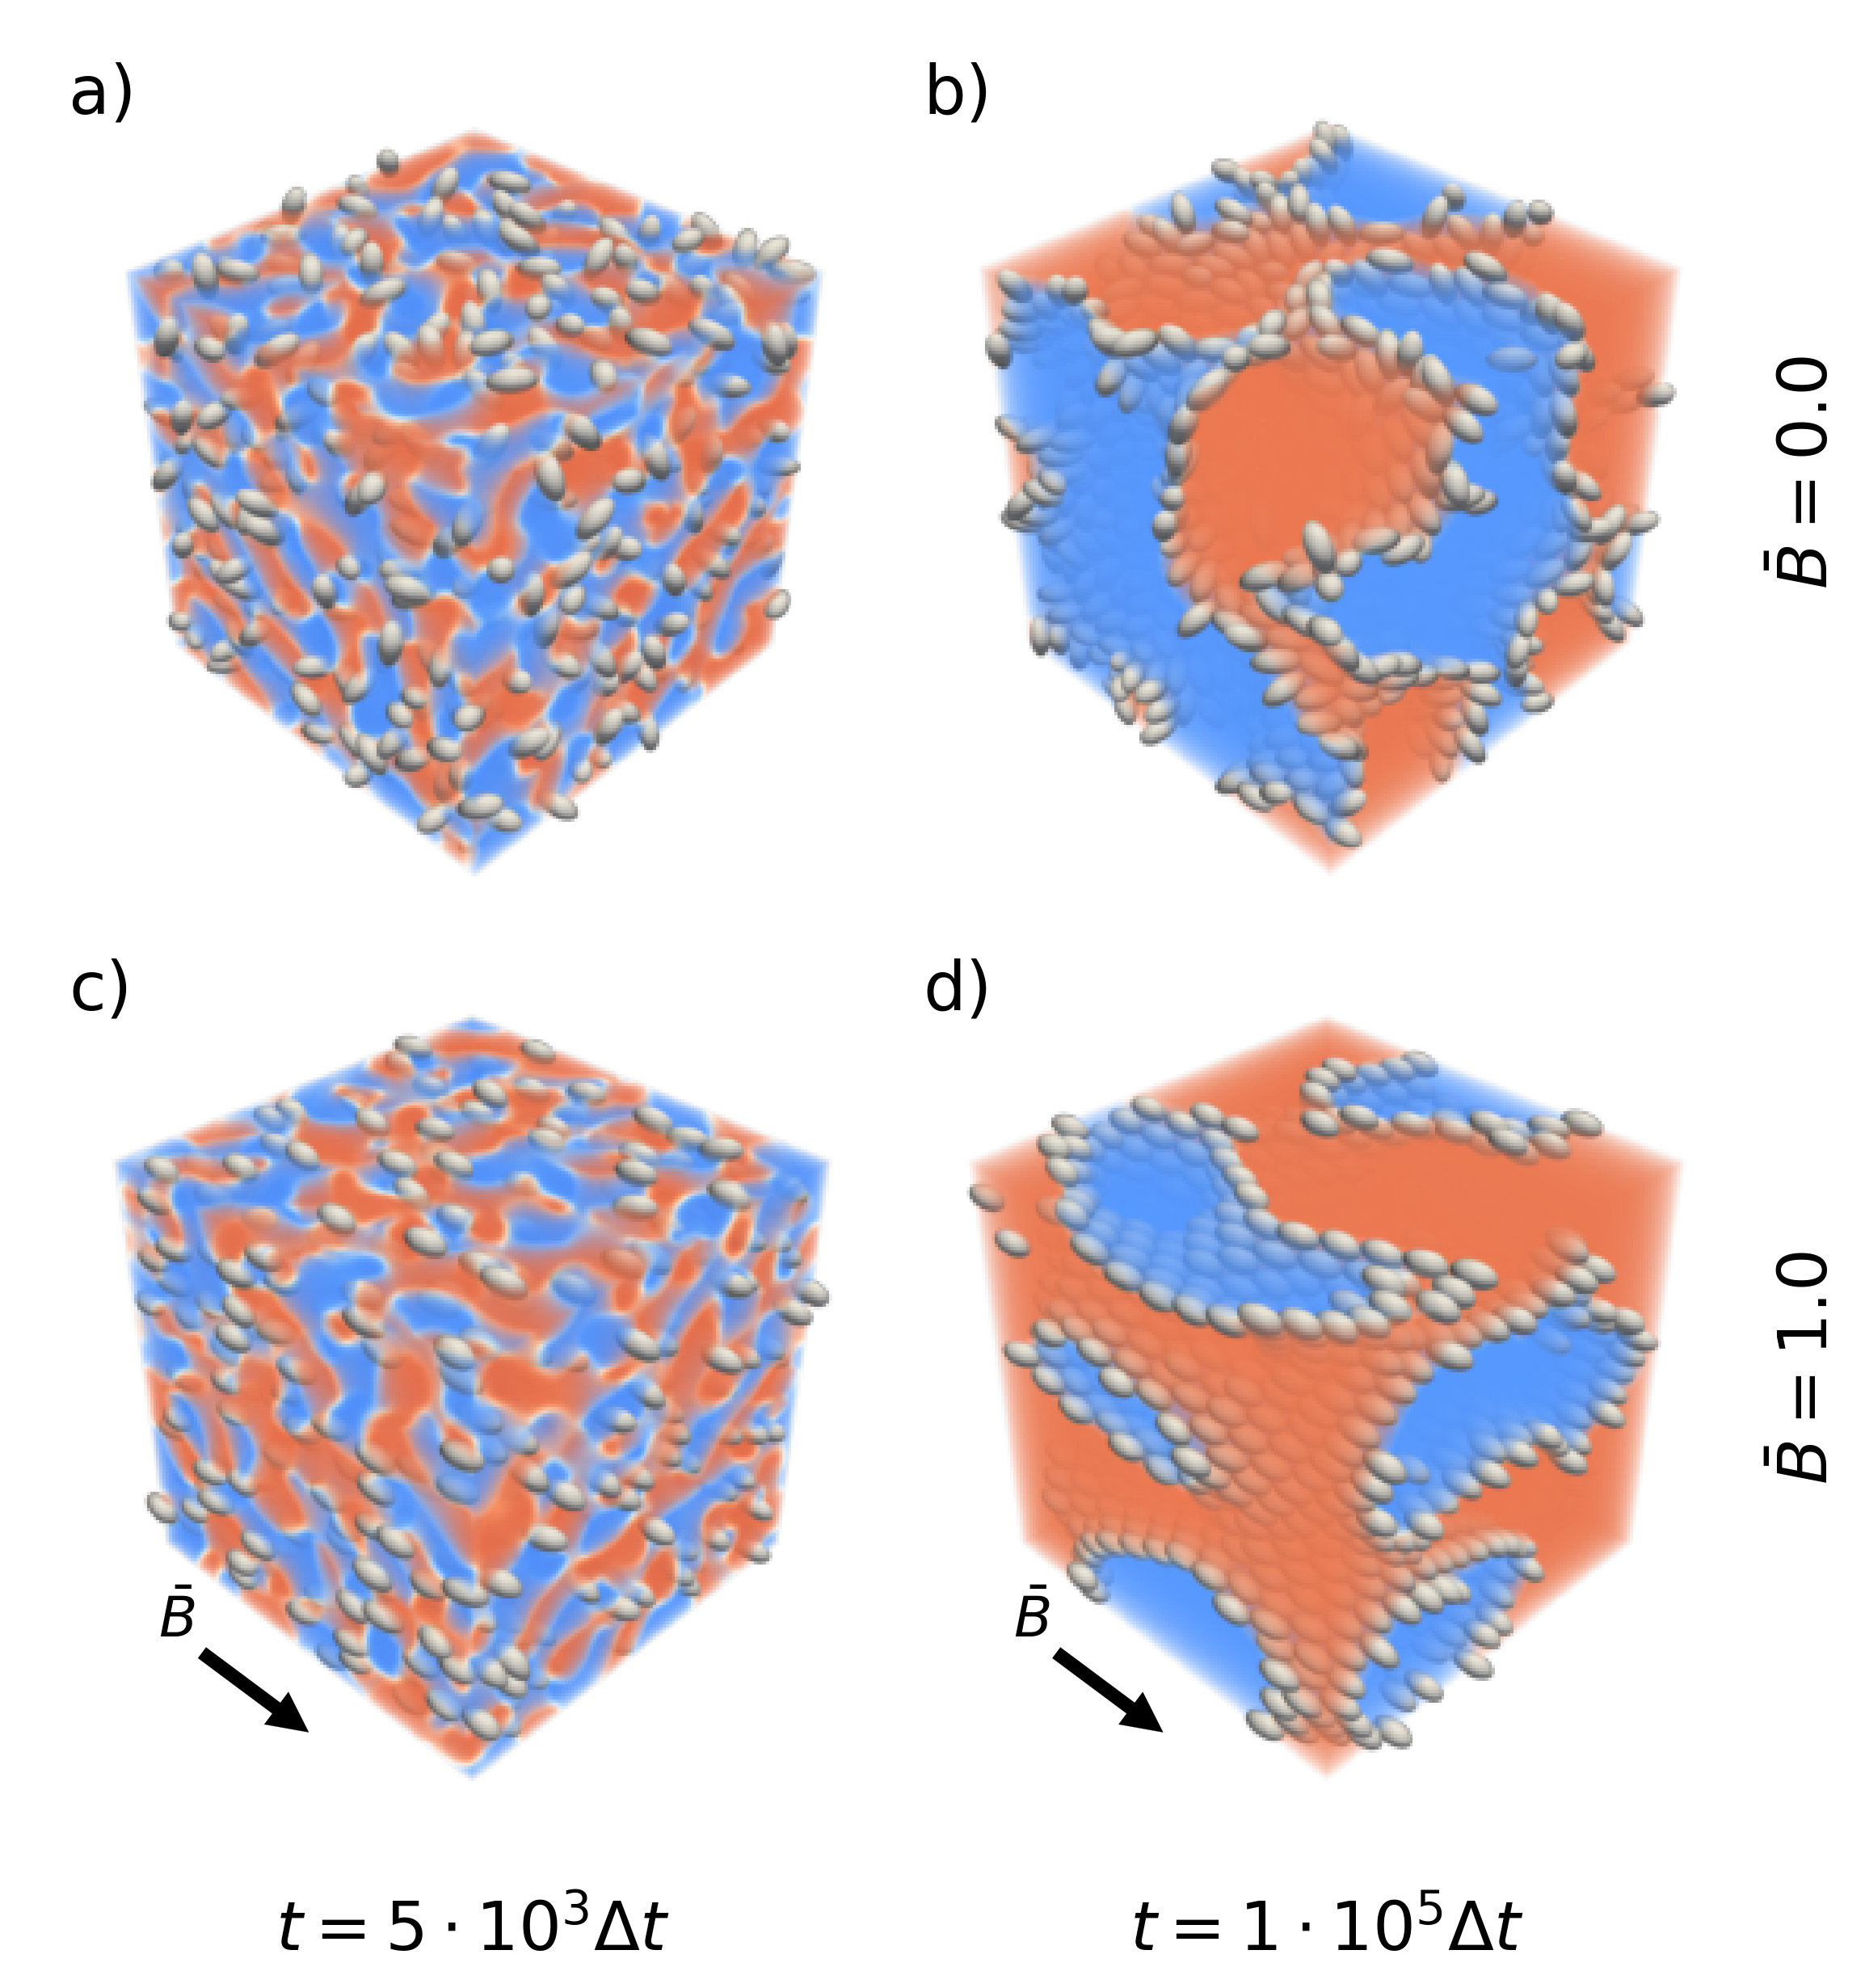
\includegraphics[width=0.5\columnwidth]{figures/results/paper1/microstructure_viz.png}
    \caption{Snapshots of emulsion gels stabilized by prolate ellipsoids after $t=5\cdot10^3$ timesteps (left) and after $10^5$ timesteps (right). The top row shows the structure forming without a magnetic field. 
             The bottom row shows the structure forming in an applied magnetic field of reduced strength $\bar{B}=1.0$. The snapshots are colored according to the order parameter $\phi$.}
    \label{fig:microstructure_viz}
\end{figure}

Figure \ref{fig:microstructure_viz} shows snapshots of the bijel
microstructure observed at different times with and without an external
magnetic field. The figure illustrates how anisotropic particles align
with the direction of the magnetic field. As the particles reorient,
they can deform the interface which thus responds by rearrangements
including reorientation and domain coalescence or breakup. This results
in apparently larger domain sizes for bijel formation in magnetic
fields. The quantitative effect on the bijel morphology, and domain size
in particular, is analyzed in the following sections.

\subsection{Structure factor and domain size of magnetically responsive bijels}

In LB simulations of spinodal decomposition, a characteristic length
scale can be obtained from the structure factor, defined in Section \ref{section:domain_size}. \cite{kendon_3d_1999,kendon_inertial_2001} 
It is worth noting that this definition of average domain size does not necessarily yield values that coincide with the typical
domain size observed visually in snapshots such as those shown in Fig.~\ref{fig:microstructure_viz}. However, in a dynamic
scaling regime, different measures of domain size are expected to differ only by a constant ratio. We found that the commonly 
used measure \(L_1(t)\) tends to overestimate the observed domain size. Numerically, the calculation of the spherically 
averaged structure factor is subject to poor statistics in the low \(k\)-shells, where the average \(|\vec{k}|\) of the 
lattice sites differs from the nominal shell radius. Additionally, the measurement of \(L(t)\) in simulations with
periodic boundary conditions is subject to finite size effects. More importantly, in suspensions of anisotropic particles, 
we cannot expect that the structure factor is isotropic. Therefore, we also used the 3D structure factor to calculate a lateral domain 
size in each Cartesian direction from the second moments also defined in Section \ref{section:domain_size}. 
\cite{jansen_bijels_2011,gunther_timescales_2014} We add the additional processing calculating a parallel and perpendicular domain size
from the results in each cartesian direction, defining $L_{\parallel}=L_z$ and $L_{\perp} = \frac{L_x+L_y}{2}$

Before calculating the structure factor \(S(\vec{k},t)\), we first filled the lattice sites covered by particles with the average
density at the surrounding lattice sites as detailed in Section \ref{section:filling_routine}. We plot the structure factor of the structures in
Figure \ref{fig:structure_factor}.

\begin{figure*}
    \centering
    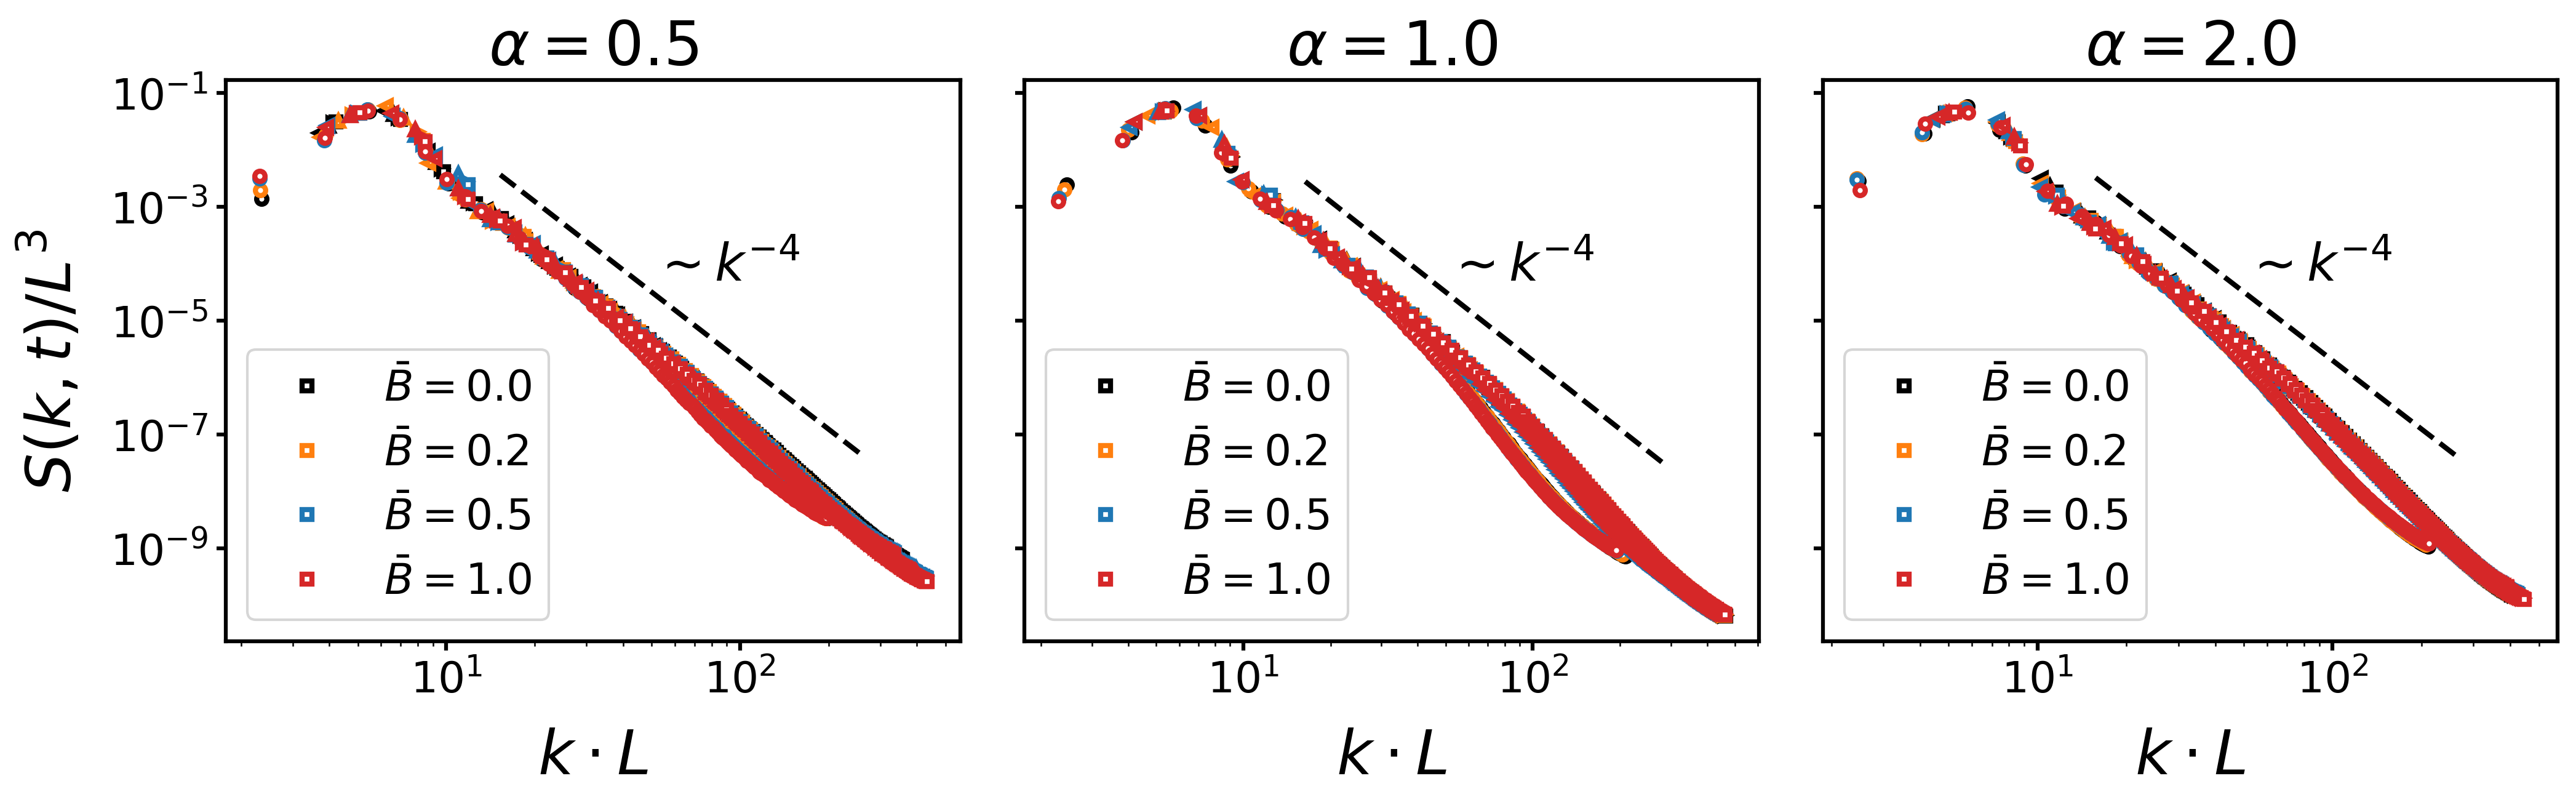
\includegraphics[width=\textwidth]{figures/results/paper1/structure_factor.png}
    \caption{Scaling plot of the dynamic structure factor $S(k,t)$ for different particle shapes $\alpha$ and at different 
            magnetic field strength $\bar{B}$. The structure factor is plotted at four different timesteps for each case. The good data collapse shows that the bijel formation is driven by spinodal decomposition. The decay to the right of the peak is reasonably well described by Porod's law $S(k)\sim k^{-4}$.}
    \label{fig:structure_factor}
\end{figure*}

Figure \ref{fig:structure_factor} shows the scaling of the dynamic
structure factor \(S(k,t)\). The data collapse is good, albeit
deviations from dynamic scaling are present at smaller length scales.
The decay to the right of the maximum is reasonably well described by
Porod's law \(S(k)\sim k^{-4}\) indicating scattering off a nearly flat
interface. These results are in line with the scaling results by Kendon
et al.~\cite{kendon_3d_1999, kendon_inertial_2001} for spinodal
decomposition of binary fluids, which suggests that the formation of
bijels is primarily driven by the separation dynamics of the fluids. The
effect of the suspended particles only comes into play once larger
domains have formed and the coarsening interface reduces the accessible
area to the point where the particles start interacting. The onset of
particle interactions and subsequent jamming leads to a fairly sudden
slow-down of domain growth, as can be observed in the time evolution of
the domain size shown in Figure \ref{fig:domain_size}.

The domain size \(L_1\) obtained from the spherically averaged structure
factor initially shows a power law behavior very close to
\(L_1\sim t^{2/3}\). A nonlinear curve fit of the function
\(b(t-t_0)^a\) to the interval \(t\in[0,\ 3\cdot10^5\Delta x]\) yields
the exponents \(a=0.6448\) for spherical particles, \(a=0.6083\) for
oblate particles with aspect ratio \(\alpha=0.5\), and \(a=0.652\) for
prolate ellipsoids with aspect ratio \(\alpha=2\). These values are in
good agreement with the exponent \(a=2/3\) that is expected in an
inertial scaling regime, where the characteristic velocity \(U=dL/dt\)
scales with the characteristic length scale
\(U\sim \sqrt{\sigma/(\rho L)}\), leading to \(L \sim t^{2/3}\). After
around 30,000 to 40,000 time steps, the domain growth starts slowing
down and approaches a plateau at \(L_1\approx 200\Delta x\) for
spherical particles, \(L_1\approx 180\Delta x\) for the prolate
particles, and \(L_1\approx 170\Delta x\) for the oblate particles.
Interestingly, the alternative domain size measure \(L_d\) obtained from
the second moments of the 3D structure factor does not show the same
power law behavior. The rate of increase of \(L_d\) is substantially
smaller than that of \(L_1\), with a fitted exponent in the range of
0.12 to 0.20. The increase of \(L_d\) levels of earlier and reaches a
plateau around \(L_d\approx 70\Delta x\) for all three particle aspect
ratios. While dynamic scaling allows different measures of the
characteristic length scale to vary by a prefactor, the deviation from
the expected power law of both viscous and inertial scaling indicates
that the second moment of the 3D structure factor does not yield a
proper characteristic length scale. %, contrary to what has been assumed in
%previous works \cite{jansen_bijels_2011, gunther_timescales_2014}.
If one interprets the moments of the structure factor as moments of a
probability distribution, then the second moment of the 3D structure
factor is equivalent to the ratio of the fourth and second moments of
the spherically averaged structure factor (due to the factor \(k^2\) in
the volume integral). Hence \(L_d\) is perhaps better interpreted as
describing the shape of the structure factor (similar to kurtosis, but
not exactly the same) rather than a characteristic length scale.
Nevertheless, the second moments \(L_\beta\) provide separate measures
for the three Cartesian directions and can thus reveal anisotropy of the
domain morphology.

\begin{figure*}
\centering
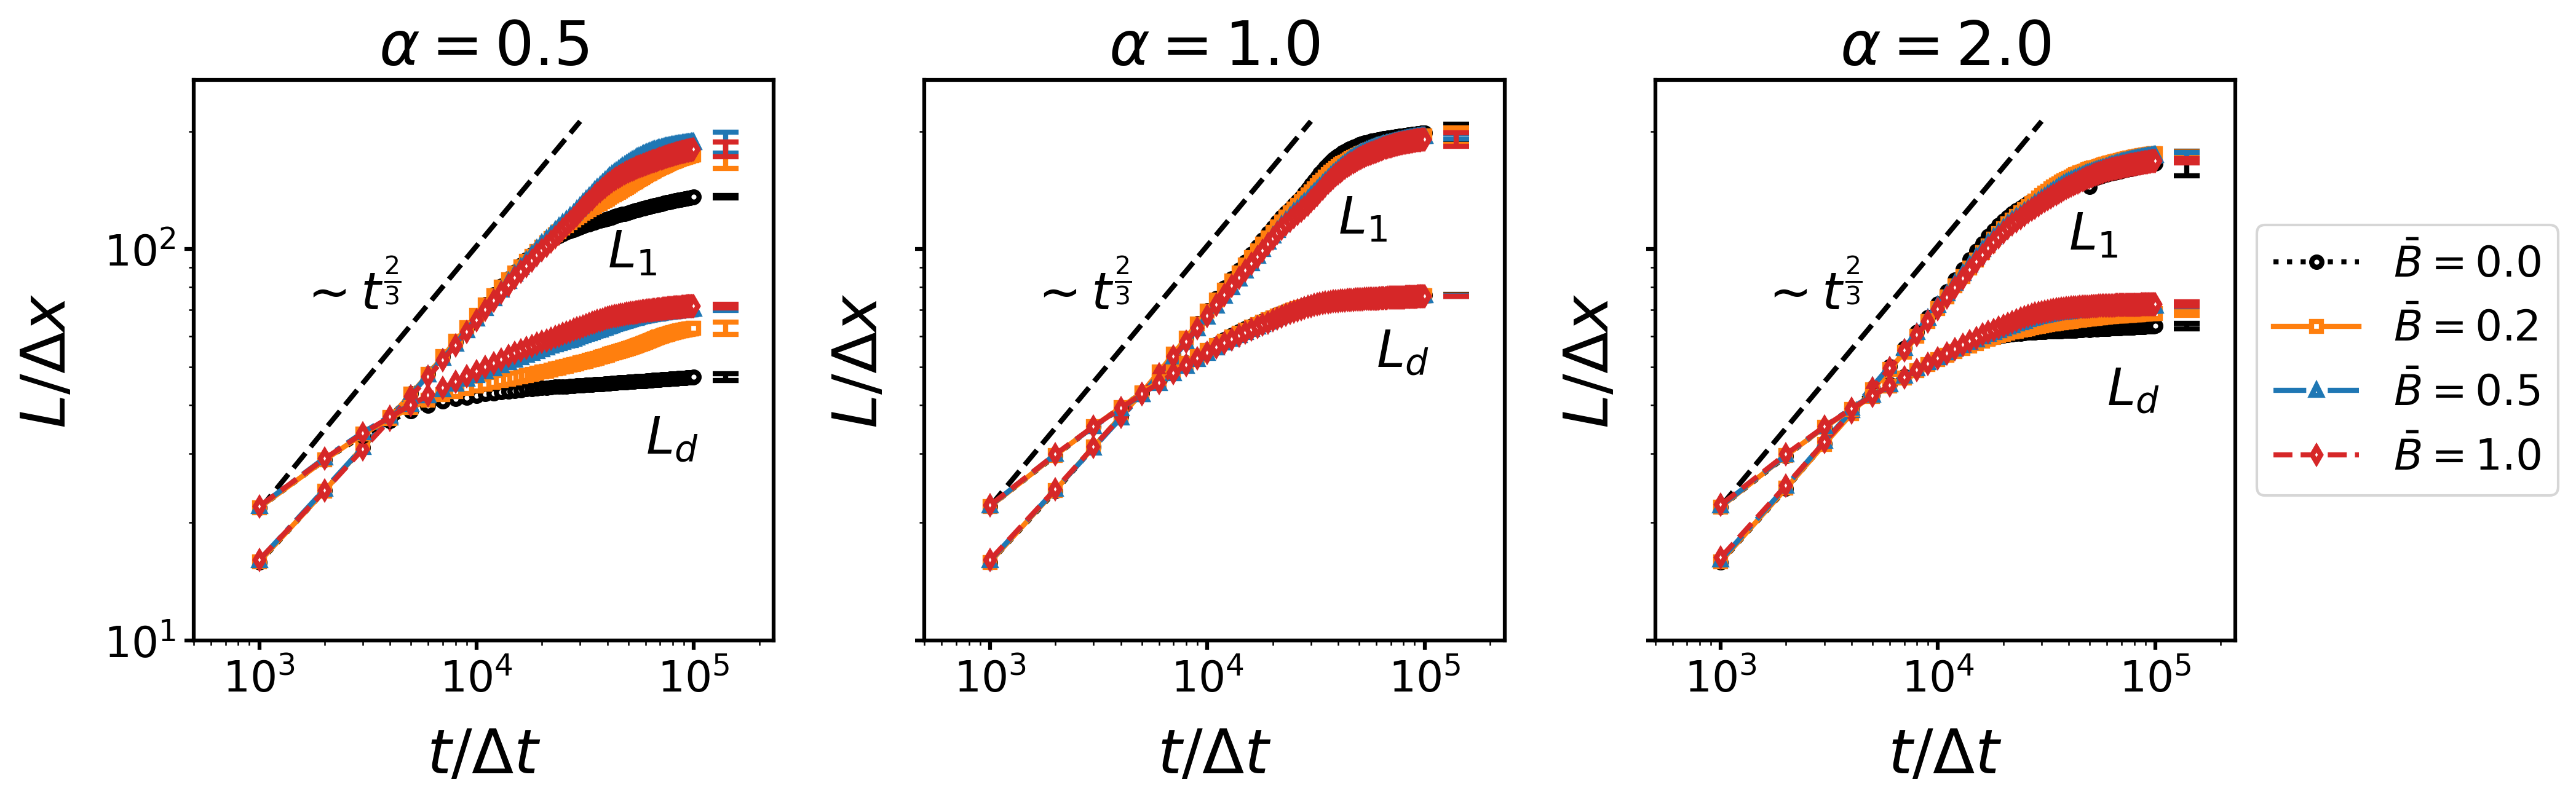
\includegraphics[width=\textwidth]{figures/results/paper1/domain_size.png}
\caption{Time dependence of the average domain size of the bijel for different particles shapes $\alpha$ and at different magnetic field strength $\bar{B}$. $L_1$ denotes the domain size obtained from the first moment of the spherical average structure factor, and $L_d$ denotes the domain size obtained from the second moment of the 3D structure factor. The increase roughly follows a $\sim t^{2/3}$ scaling law indicative of the inertial regime of spinodal decomposition.}
\label{fig:domain_size}
\end{figure*}

\subsection{Effect of magnetic field on bijel formation}

\begin{figure}
\centering
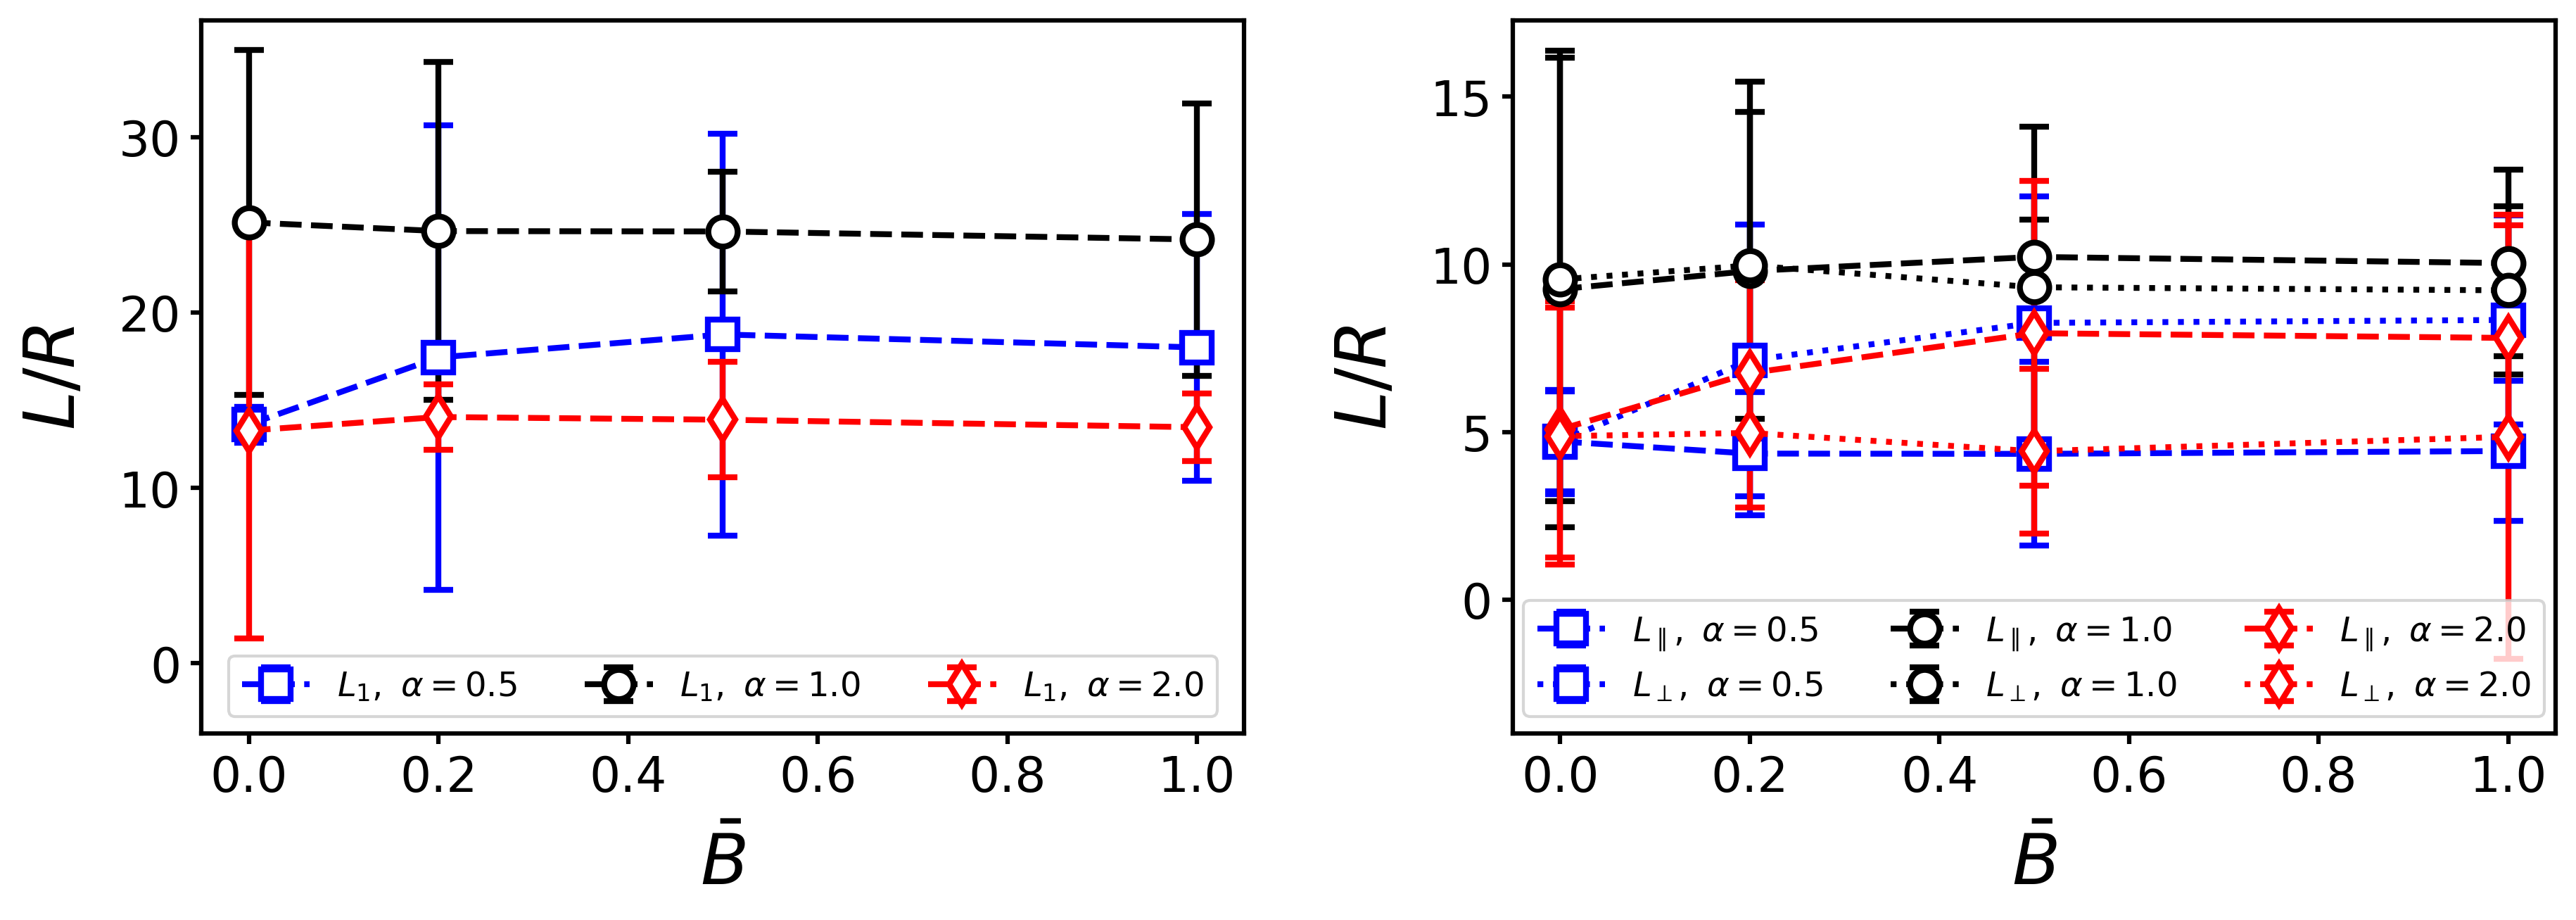
\includegraphics[width=\columnwidth]{figures/results/paper1/D2a-vs-B_ss.png}
\caption{Dependence of the average domain size on the magnetic field strength $\bar{B}$. The left plot shows the average domain size $L_1$ obtained from the spherically averaged structure factor. The right plot shows the parallel and perpendicular domain size obtained from the respective second moments of the 3D structure factor. Errorbars indicate the standard deviation taken over three independent simulation runs. For anisotropic particles, the directional domain size becomes more anisotropic with increasing field strength.}
\label{fig:D2a_B}
\end{figure}

At first glance, the time-dependence of the domain size in Fig.
\ref{fig:domain_size} suggests that the domain size is not strongly
affected by the external magnetic field. In Fig.\ref{fig:D2a_B}a) we
plotted the domain size measure \(L_d\) normalized by \(R\), the larger
of the two radii of the ellipsoidal particles. The data points represent
the domain size measured at the final time step and averaged over three
independent simulation runs with the same parameters. The normalization
with the particle radius makes it apparent that the ellipsoidal
particles reduce the domain size of bijels. This observation is in line
with observations by Günther et al.~\cite{gunther_timescales_2014} and
indicates that -- relative to their volume -- ellipsoidal particles
stabilize a larger interface area than spherical particles. This is due
to the larger cross-sectional area of ellipsoidal particles at the same
volume. Furthermore, steric constraints prevent anisotropic particles to
pack less densely in the interface than spherical particles, as we will
discuss in more detail below.

The magnetic field does have an effect on the directional
domain size as shown in Figure \ref{fig:D2a_B} where we plotted the
domain size in the direction parallel and perpendicular to \(\vec{B}\)
separately. We find that for prolate particles, the domain size in the
parallel direction increases with the field strength up to approximately
three particle radii for the largest field, while the perpendicular
domain size stays constant. This trend is reversed for oblate particles
for which the domain size in the parallel direction decreases slightly
with field strength while the perpendicular domain size increases by
approximately four particle radii. Without a field, prolate
particles lead to smaller domain size than both spherical and oblate
particles, whereas they increase the domain size when the bijel forms under the
influence of a magnetic field. The anisotropy is due to the alignment of
ellipsoidal particles which leads to a closer packing within the
interface akin to nematic ordering. The difference between oblate and
prolate particles is caused by the orientation of the magnetic dipole
moment \(\vec{m}\) along the symmetry axis of the particles. In our
model, \(\vec{m}\) is aligned with the larger axis of prolate
ellipsoids, whereas it is aligned with the smaller axis of oblate
ellipsoids. Hence \(\vec{m}\) lies in the plane of the larger
cross-section of prolate particles while \(\vec{m}\) is perpendicular to
the larger cross-section of oblate particles. We thus expect that
alignment of the particles with the magnetic field \(\vec{B}\)
facilitates closer packing perpendicular to the field for prolate
particles, and parallel to the field for oblate particles. The
increase/decrease of domain size levels off at intermediate field
strength and further increases of the field have no additional effect.

\subsection{Tortuosity}

\begin{figure*}
\centering
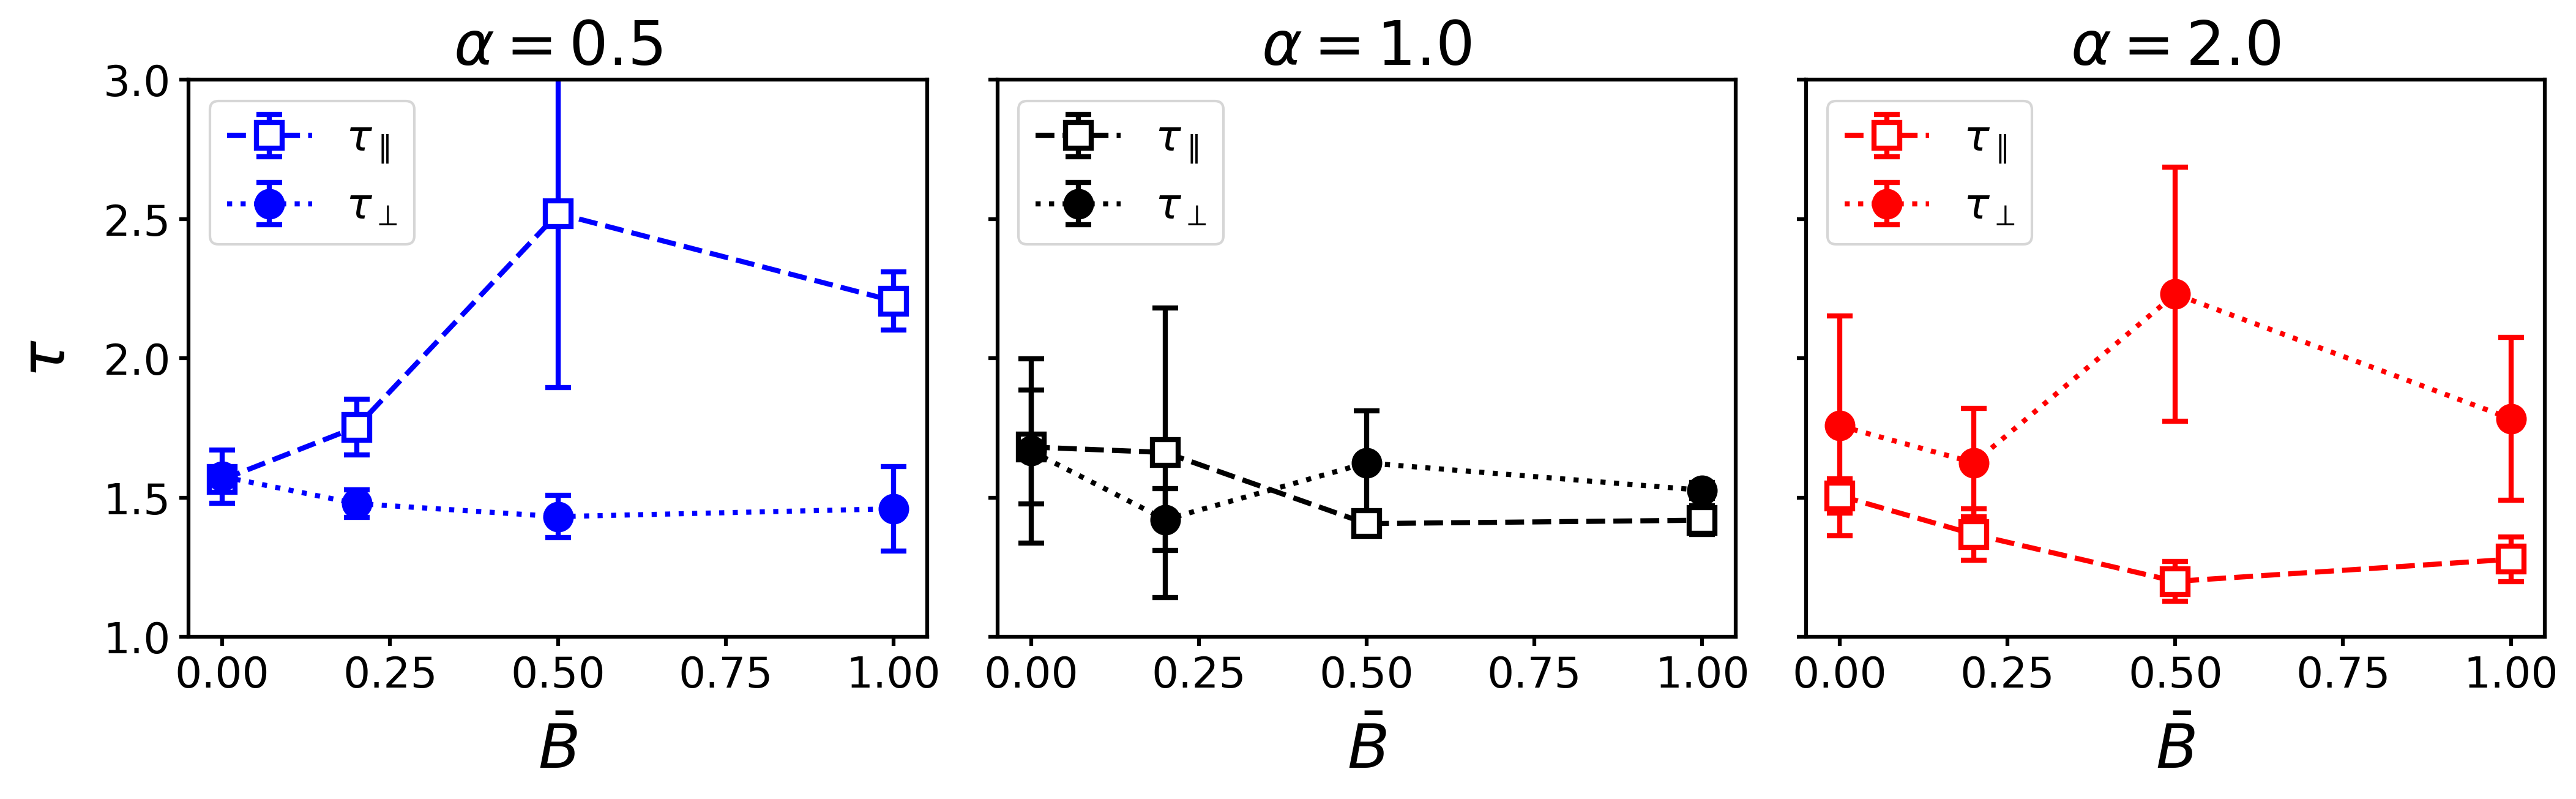
\includegraphics[width=\textwidth]{figures/results/paper1/tortuosity_compare.png}
\caption{Dependence of the tortuosity on the magnetic field strength $\bar{B}$ for different particle shapes $\alpha$. 
Different components of the tortuosity tensor show the anisotropy for oblate and prolate particles.}
\label{fig:tau_B}
\end{figure*}

The anisotropy of domain size suggests that the magnetic field
influences the bijel morphology at the microscale. To investigate
whether these structural changes have an effect on macroscopic
transport properties, we also characterized the tortuosity of the
bijels. Various definitions of tortuosity have been proposed in the
literature \cite{dasilva_tortuosity_2022}, including geometric,
diffusional, and hydraulic tortuosity. Here we use the diffusional
tortuosity $\tau= \frac{\epsilon D}{D_{\text{eff}}}$, i.e., the ratio of the 
effective diffusivity $D_{\text{eff}}$ and the intrinsic diffusivity
$D$. We calculate the tortuosity using the procedure detailed in Section \ref{section:tortuosity}

Figure \ref{fig:tau_B} shows the results for the tortuosity as a
function of the applied magnetic flux for the three particle aspect
ratios. In the absence a magnetic field, the three aspect ratios lead to
a similar tortuosity around $\tau\approx 1.5$, slightly larger than
the tortuosity predicted by the Bruggeman relation
\(\tau=\epsilon^{-0.5}=1.41\) for equal volume fractions
\(\epsilon=0.5\) of the phases
\cite{bruggeman1935tortuosity, tjaden_origin_2016}. The observed
tortuosity is consistent with simulations of gyroid structures by Luo et
al., who found diffusive tortuosities in the range from 1.48 to 1.73
\cite{luo_macroscopic_2020}. Figure \ref{fig:tau_B} shows that in an
applied magnetic field, the tortuosity of bijels stabilized by
anisotropic particles (\(\alpha\neq1\)) becomes anisotropic as well.
Oblate particles (\(\alpha=0.5\)) lead to an increase of the tortuosity
\(\tau_\parallel\) in the direction of the magnetic field while the
tortuosity in the direction perpendicular to the magnetic field remains
around \(\tau_\parallel\approx1.5\). Conversely, prolate particles
(\(\alpha=2\)) lead to an increase of the tortuosity in the direction
perpendicular to the magnetic field, while the tortuosity in the
parallel direction slightly decreases with increasing field strength. In
both cases, the changes in tortuosity are consistent with the
anisotropic domain size and the alignment of particles with the magnetic
field. For prolate particles, the longer axis is aligned with the
magnetic moment and induces larger domain size and lower tortuosity in
this direction. The results show that the magnetic field has a
noticeable effect on the tortuosity of the bijel. We observe that the
largest change of tortuosity is measured at intermediate field strength
\(\bar{B}=0.5\). This suggests that the competition of interfacial and
magnetic forces and the resulting alignment of particles and liquid
domains induces morphological changes that are more complex than a
monotonic increase or decrease. We therefore turn to investigate the
microstructural changes within the bijel morphology in more detail.

\subsection{Curvature}

Beyond the length scale, curvature analysis offers insights into the
local topological landscape of the bijel, facilitating further
microstructure optimization for various applications.
\cite{reeves_quantitative_2016} We plot the area averaged mean and
gaussian curvature \(H\Sigma^{-1}\) and \(K\Sigma^{-2}\) for bijels
stabilized with oblate, spherical and prolate ellipsoids in Figure
\ref{fig:curvature-vs-B_ss}. 

\begin{figure} 
    \centering 
    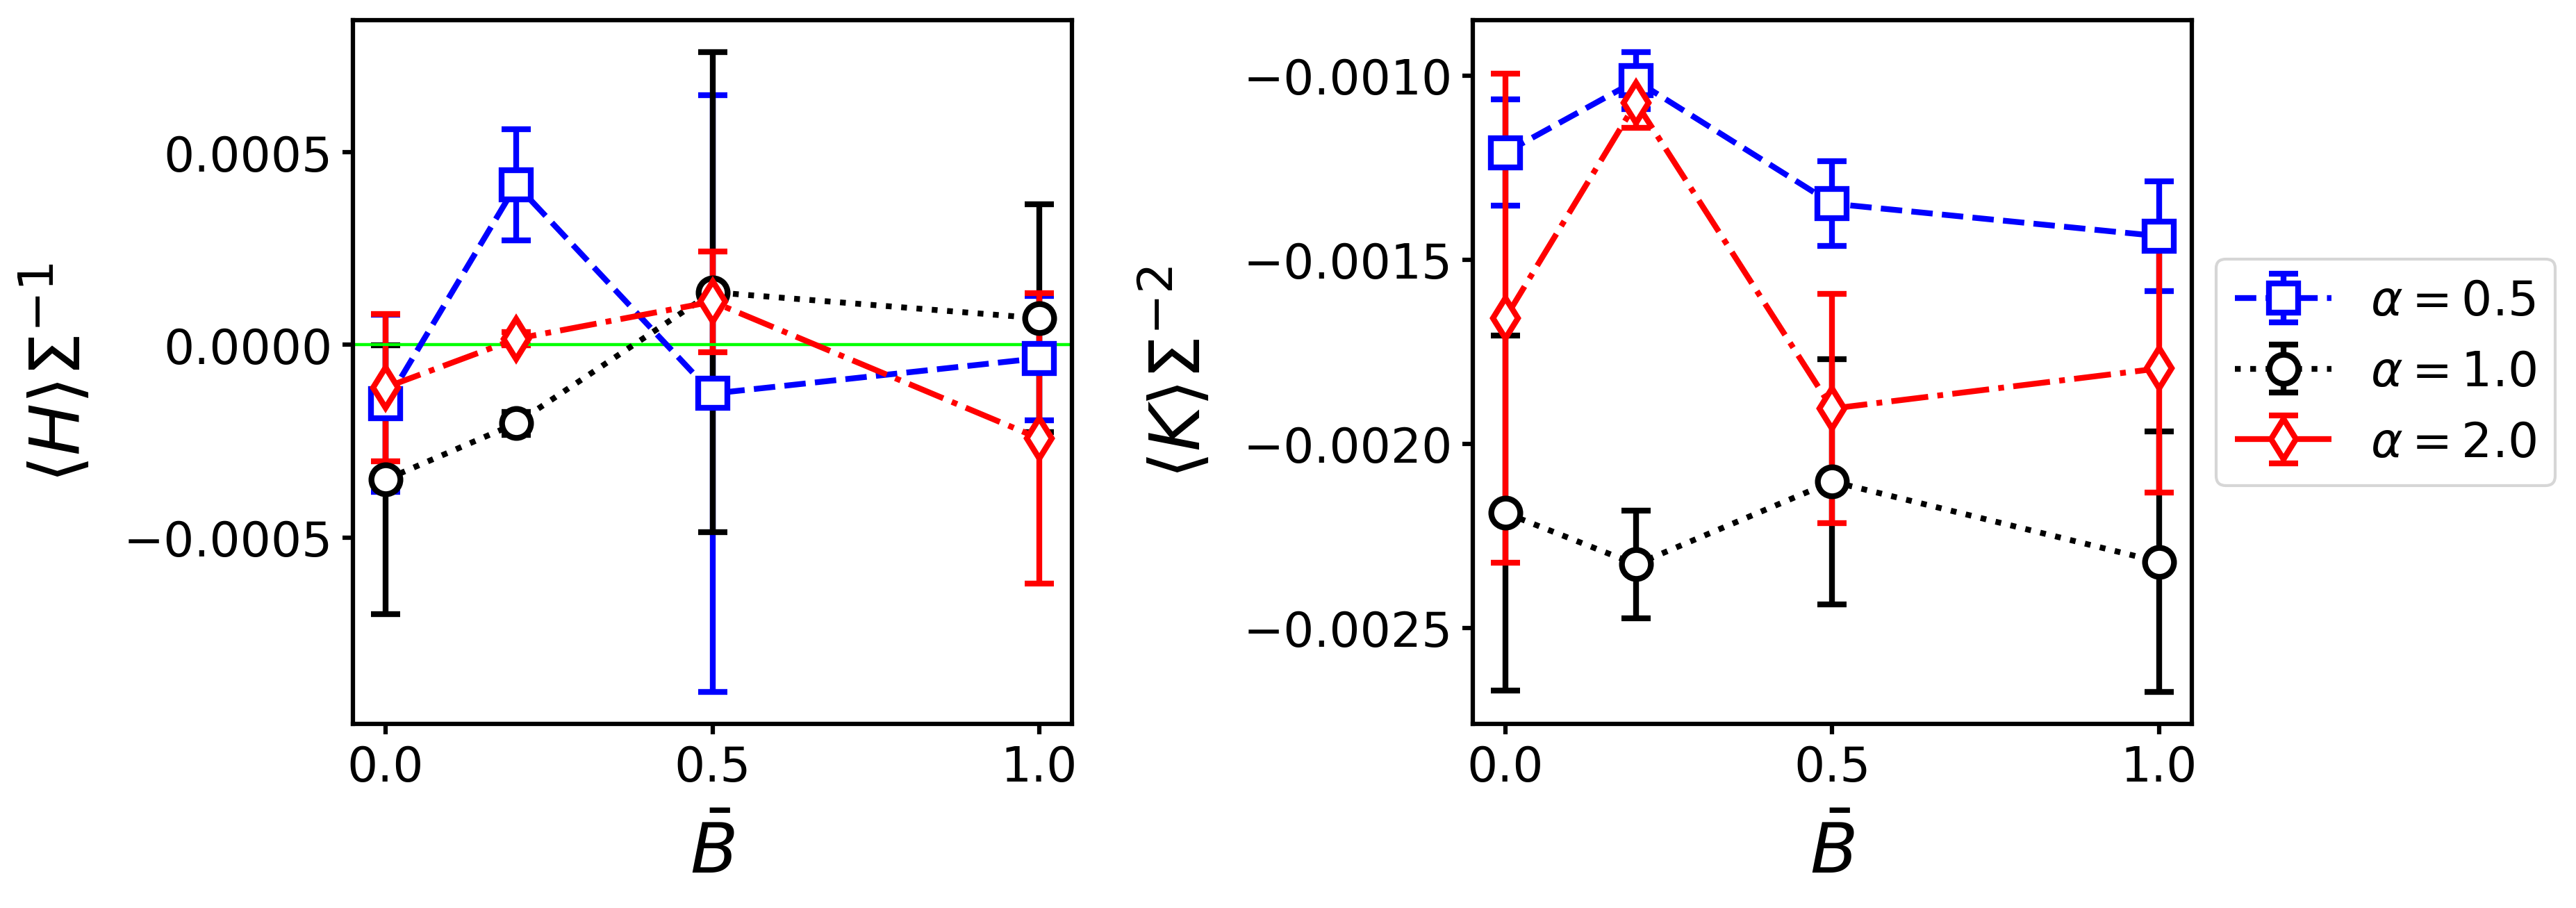
\includegraphics[width=\textwidth]{figures/results/paper1/curvature-vs-B_ss.png} 
    \caption{Plot of the area averaged mean $\langle H \rangle \Sigma^{-1}$ and Gaussian 
            $\langle K \rangle \Sigma^{-2}$ curvature in the left and right respectively. Each 
            plot contains the $\langle H \rangle \Sigma^{-1}$ and $\langle K \rangle \Sigma^{-1}$ 
            at the final timestep averaged across 3 runs for particles with $\alpha = 0.5, 1, 2$. 
            We observe that the mean curvature does not demonstrate any trends, while the Gaussian 
            curvature shows a reduction as the magnetic field strength is increased for 
            ellipsoidal particles.} 
    \label{fig:curvature-vs-B_ss}
\end{figure}

Error bars are represented by the standard
deviation of the three simulations per parameter set performed. The area
averaged mean curvature shows little dependence on the applied field
strength with values around 0 and within error of one another. A value
near or at 0 is expected as the fluid volume fraction is equal and the
particles are neutrally wetting, implying the interface should not have
a preferred direction of curvature. \cite{jinnai_interfacial_2001} For
ellipsoidal particles, the gaussian curvature becomes more negative as
larger field strengths are applied. We also see that the gaussian
curvature becomes more positive as the interfacial area of the particle
increases. The trend of these results are inverse to the interfacial
area of each particle, \(A_{rm}\). This is expected behavior and is in
agreement with experiments that have investigated the effect of particle
size on the curvature of bijels. \cite{reeves_quantitative_2016}

Reeves and coworkers identified that nanoparticles were better able to
lock in the spinodal structure of the liquid-liquid phase separation as
they were less disruptive the the curvature of the interface due to
their lower interfacial adsorption energy. This effect can be observed
as a more negative Gaussian curvature as a result of the greater number
of hyperbolic surfaces, a hallmark of a minimal surface. In our system,
the oblate and prolate particles have 60\% and 30\% more interfacial
area than the spherical particles, resulting in the ellipsoidal
particles being more disruptive to the curvature of the interface,
observed as a more positive Gaussian curvature. As the magnetic field
strength is increased, the packing of the particles at the interface
changes, as observed from the radial distribution function.
\cite{karthikeyan_formation_2024} These changes in particle packing
change the way the particles affect the curvature of the interface,
resulting in the curvature changes observed. To investigate the field
dependence on the curvature, we plot the area averaged Gaussian
curvature as a function of time.

\begin{figure} 
    \centering 
    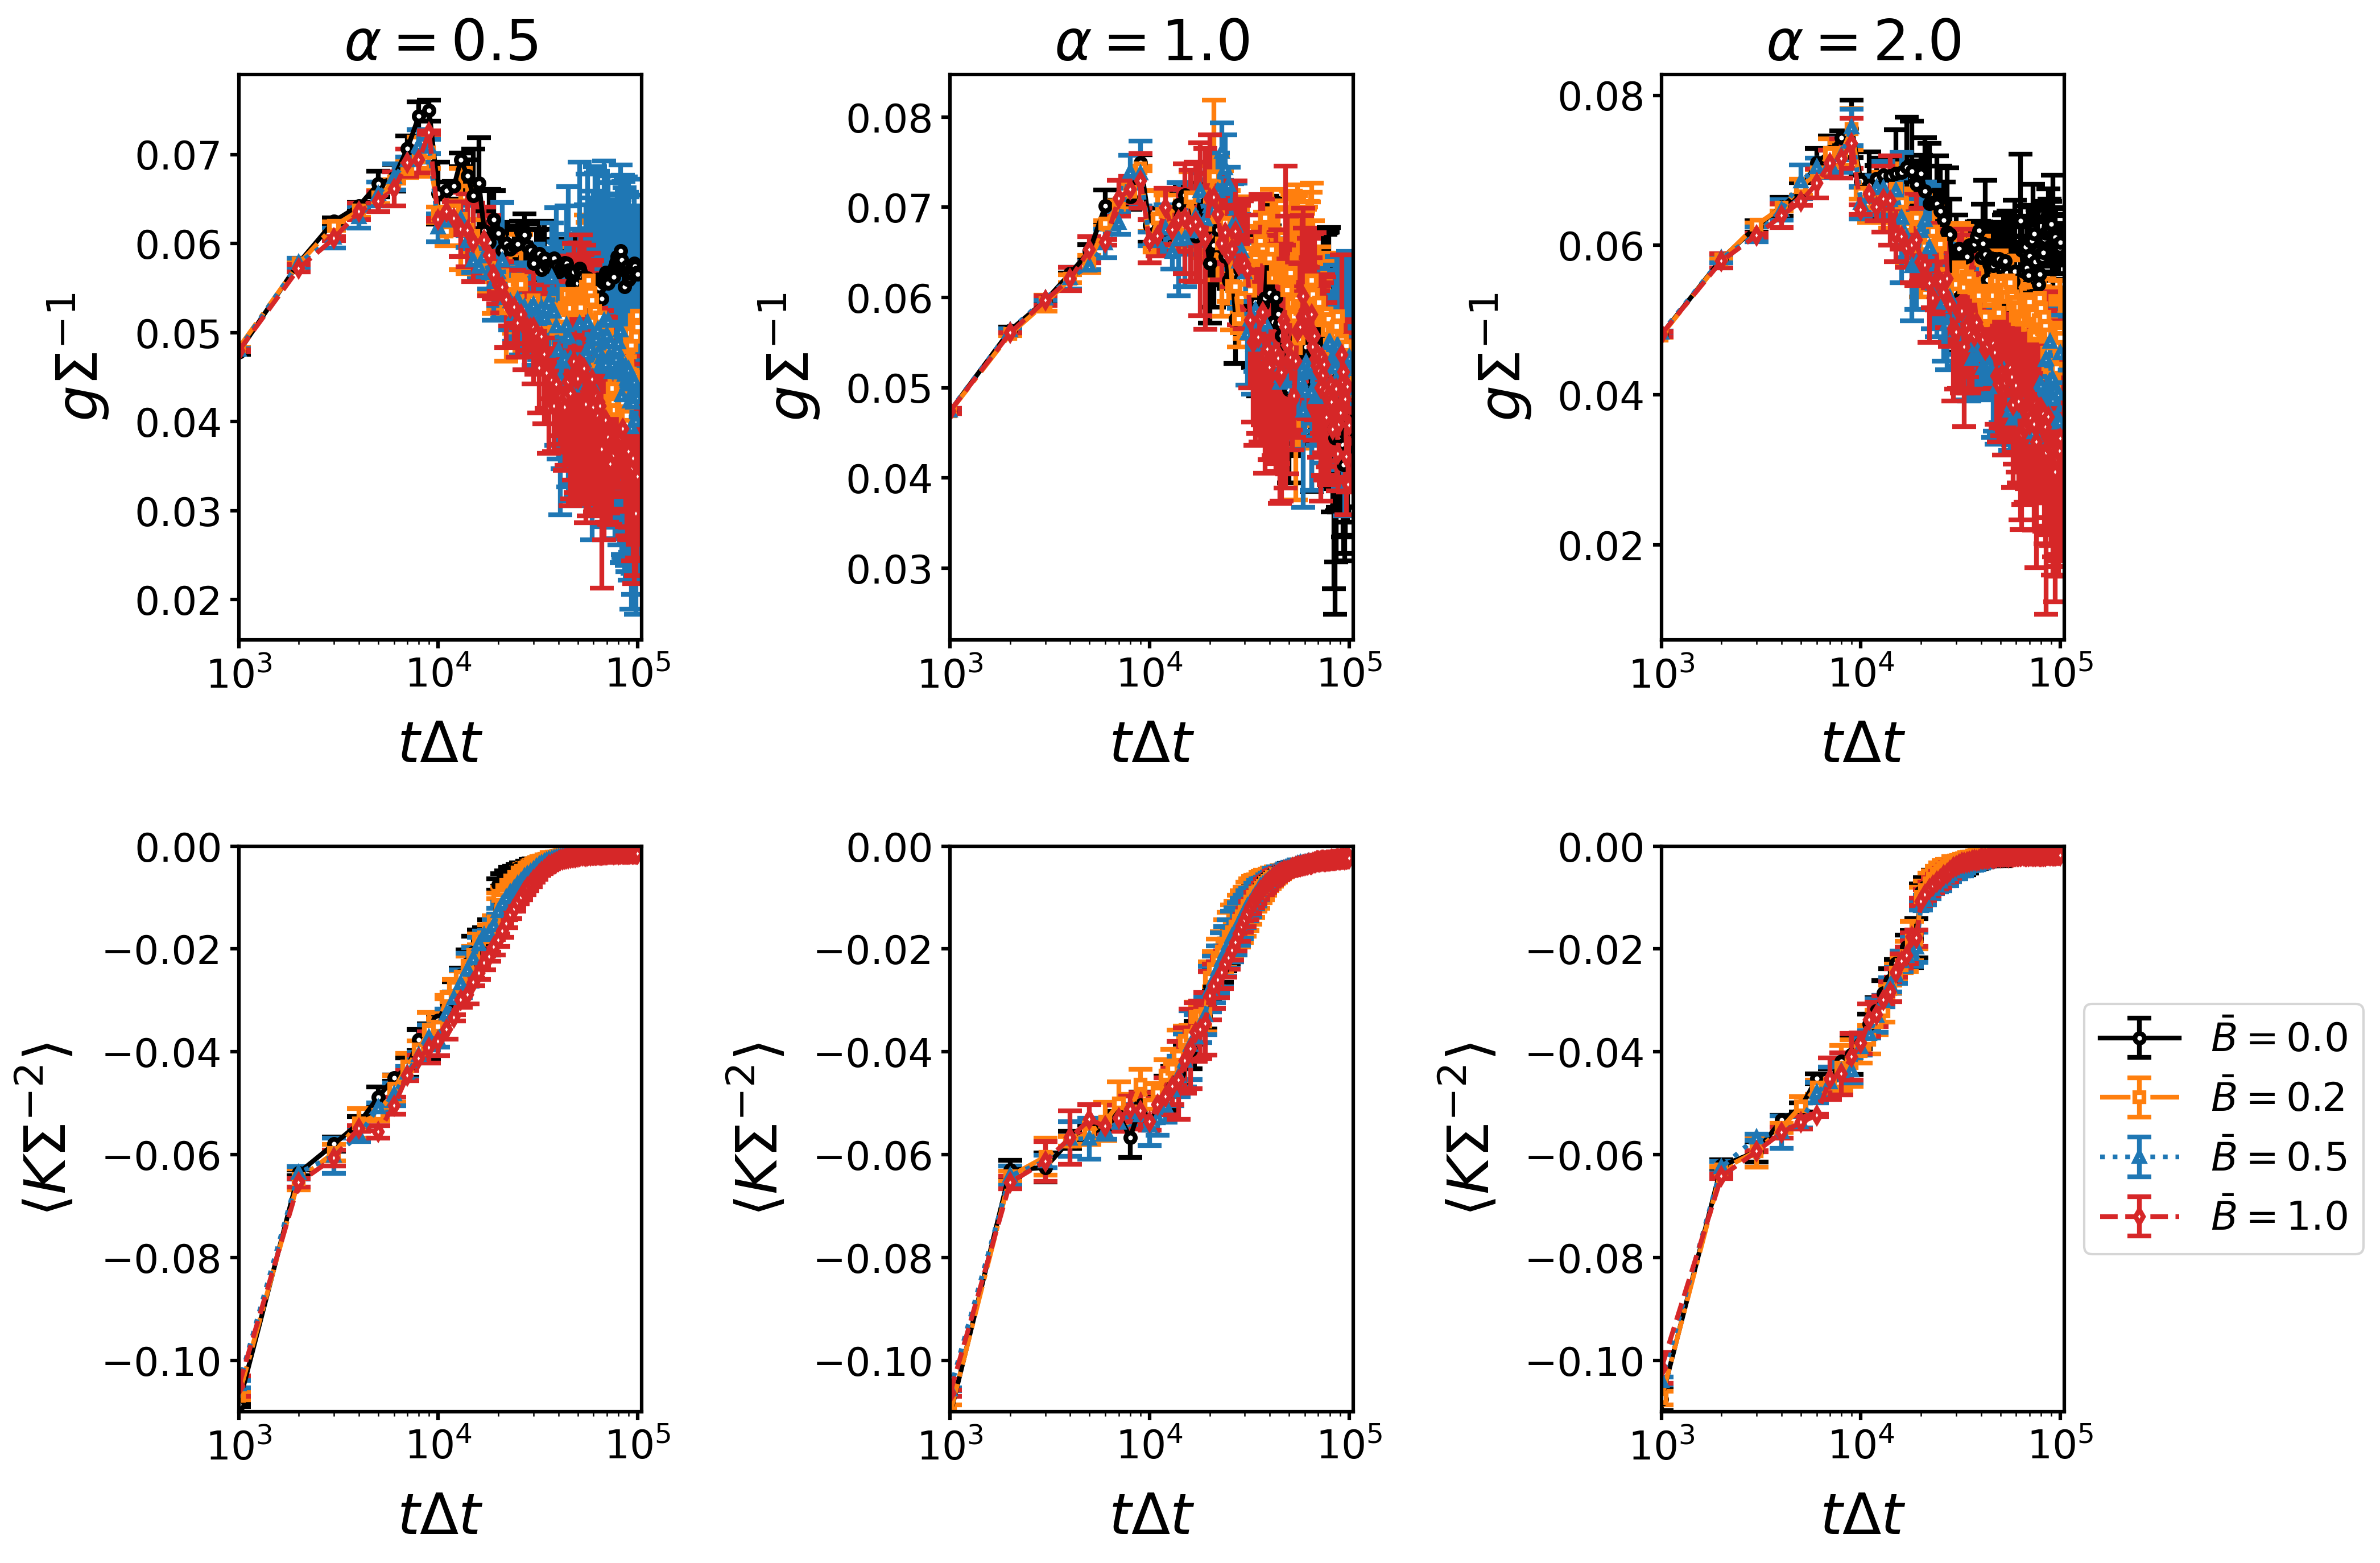
\includegraphics[width=\textwidth]{figures/results/paper1/genus_curvature_vs_coverage.png} 
    \caption{Plots of Gaussian $\langle K \rangle \Sigma^{-2}$ curvature over time averaged across 3 runs. 
    From left to right, we have particles with $\alpha = 0.5, 1, 2$. We observe that the initial stages of 
    evolution are unaffected by the applied magnetic field. However, after about 10000 timsteps, we see a 
    magnetic field dependence on the evolution of the Gaussian curvature. The preservation of this divergence 
    occurs when ellipsoidal particles are used but not spherical particles.} 
    \label{fig:curvature_vs_coverage}
\end{figure}

Given we did not see any noteworthy changes in the mean curvature in
Figure \ref{fig:curvature-vs-B_ss}, we focused on the Gaussian curvature
in Figure \ref{fig:curvature_vs_coverage}. We observe that for all
simulated systems, the Gaussian curvature increases over time until an
invariance is reached near the end of the simulation, signifying the
bijel microstructure is locked in place. We also observe that for all
microstructures the curvature over time does not increase at the same
rate, characterized with dips at 10 to 20,000 timesteps for all
particles and a magnetic field dependent change in the curvature
increase.

However, for the spherical particles this local topology change
disappears once the spinodal decomposition ceases, observed as a
convergence of all curvatures. This is not observed for the bijels
stabilized by ellipsoidal particles. Despite all our curvature
calculations being normalized with their surface area to volume ratio,
we still see curvature differences as a function of the applied magnetic
field. Experiments have identified that curvature changes can occur due
to the formation of monogels, which are particle networks formed from
bijels that can withstand the remixing of their constituent liquids.
\cite{sanz_colloidal_2009, lee_making_2013} This process cannot occur in
our simulations as we are utilizing repulsive particles. Therefore, the
change in curvature arises from the differences in local state of the
colloids at the interface.

\subsection{Kinetics of bijel formation in magnetic fields}

To shed light on the mechanisms involved in the coarsening dynamics,
we now turn to the kinetics of bijel formation in more detail. The
coarsening dynamics can be characterized by a coarsening speed. Here,
we use the finite difference of the directional domain size to
calculate the components of the coarsening velocity
%
\begin{equation}
u_{L_\beta}(t) = \frac{L_\beta(t+\Delta t_s)-L_\beta(t-\Delta t_s)}{2\Delta t_s} ,
\end{equation}
%
where \(\Delta t_s\) is the time between simulation
snapshots, and $\beta$ denotes either the direction parallel or perpendicular to the magnetic field.

\begin{figure*}
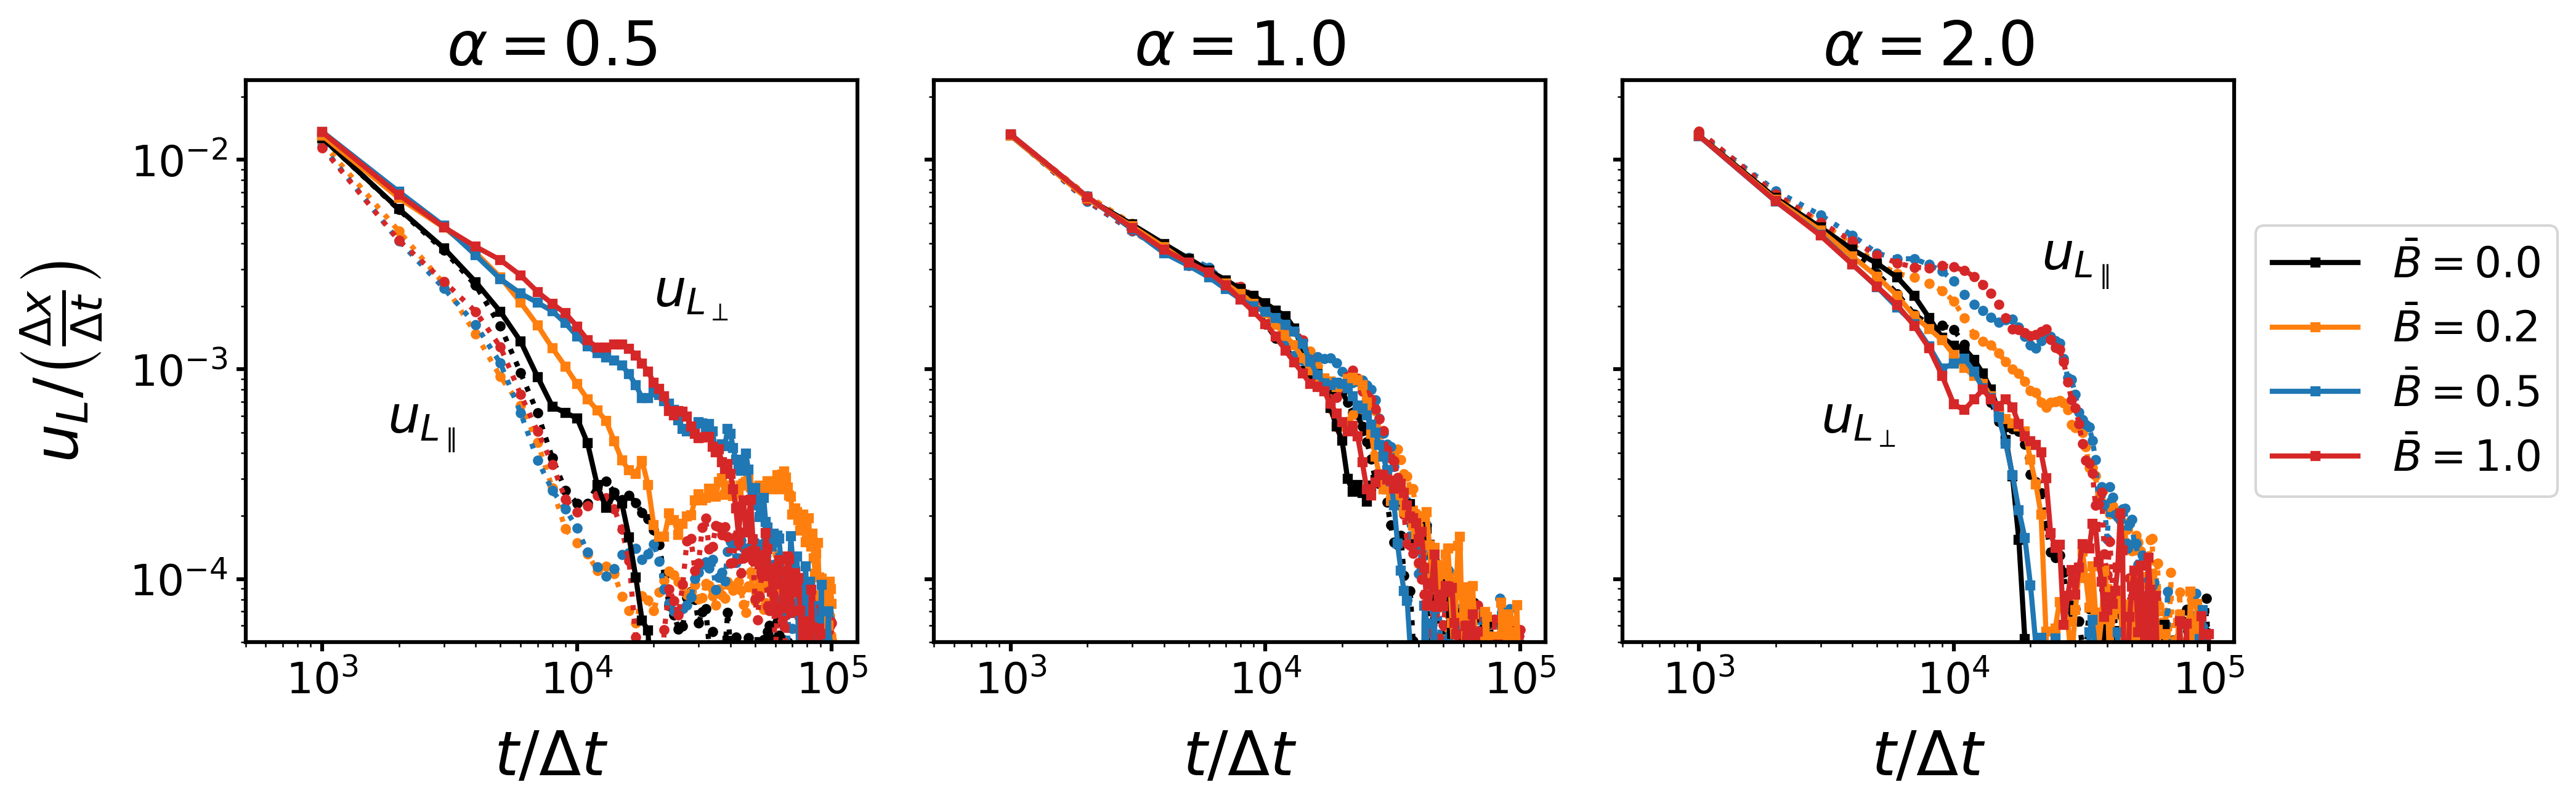
\includegraphics[width=\textwidth]{figures/results/paper1/coarsening_vel.png}
\caption{Time-dependence of the coarsening velocity $u_L$ for different particles shapes $\alpha$  
and at different magnetic field strength $\bar{B}$. The different components of the coarsening velocity 
show that the jamming time is different in the direction parallel and perpendicular to the magnetic field.}
\label{fig:coarsening_velocity}
\end{figure*}

Figure \ref{fig:coarsening_velocity} shows the coarsening speed in the directions parallel and perpendicular to the applied magnetic field. The data confirms that for spherical particles, domain coarsening remains isotropic. We observe a higher coarsening speed initially which slows at later times when the particles begin to jam. This indicates that the
coarsening is subject to different time scales, as reported previously
by Harting and co-workers \cite{gunther_timescales_2014}. Reeves et
al.~\cite{reeves_particle-size_2015} have pointed out that bijel
formation hinges on the jamming time in relation to the disruption time, i.e., the time scale at which domain pinch-off events can cause bijel break-up through depercolation. In our simulations, however, we have not observed disruption of bijel formation; stable bijels form for all parameters consistent with simulations by Stratford et
al.~\cite{stratford_colloidal_2005} and Jansen et al.~\cite{jansen_bijels_2011}.

For ellipsoidal particles, our data clearly shows that an\-isotropic
domain coarsening arises in magnetic fields.  For oblate particles
(\(\alpha=0.5\)), the coarsening speed in the direction perpendicular
to the field increases with increasing magnetic field strength.
Jamming in this direction appears to be delayed compared with the
direction parallel to the field. The coarsening speed in the parallel
direction remains comparable to the case without an applied magnetic
field. This anisotropic behavior of the coarsening speed reverses for
prolate particles, where the coarsening speed in the direction parallel to the field increases with increasing field strength, and jamming in this direction
is delayed compared with the perpendicular direction. In addition, we observe a shoulder (around \(10^4\Delta t\)) where the coarsening speed decays more slowly before jamming sets in. These results suggest that the coarsening near the jamming time is affected by a mechanism that depends on the applied magnetic field and causes the anisotropic
behavior. This mechanisms involves the re-orientation of anisotropic
particles and their alignment relative to the direction of the
magnetic field. To confirm this hypothesis, we analyze the
orientational order of the particles and their alignment relative to
the magnetic field and the interface, respectively.

\subsection{Particle re-orientation and packing}

\begin{figure}
\centering
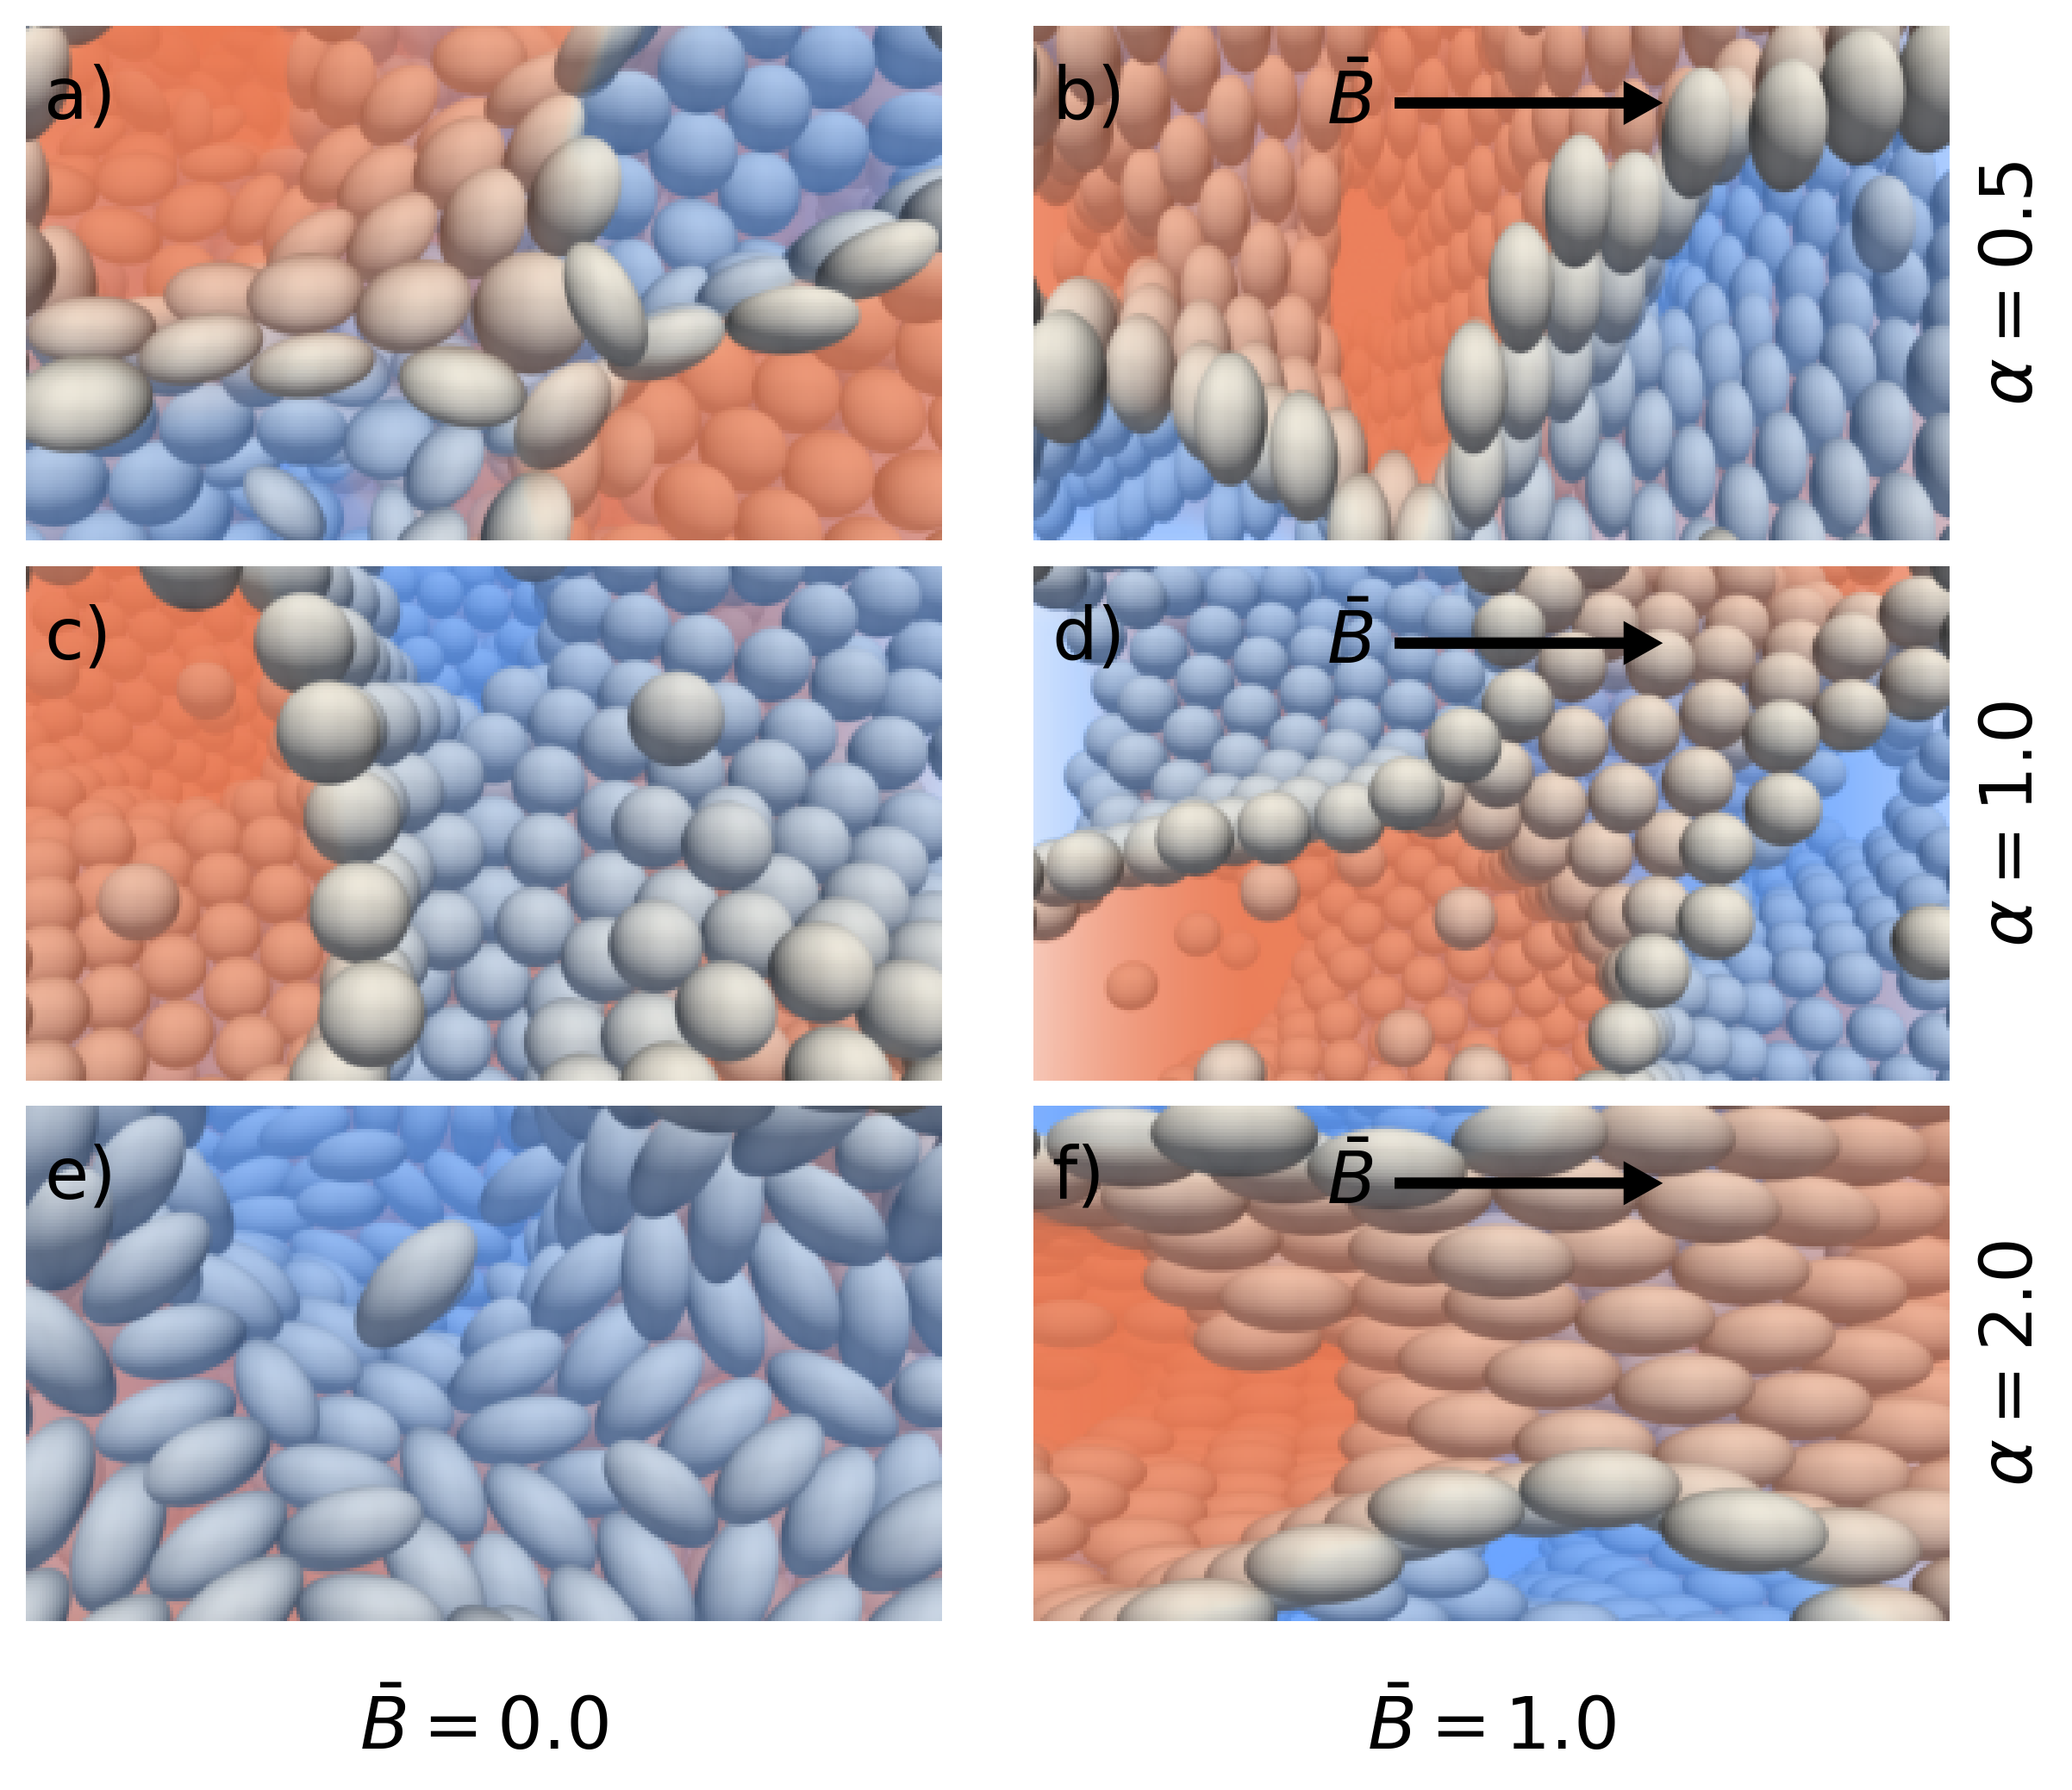
\includegraphics[width=0.5\columnwidth]{figures/results/paper1/particle_packing_viz.png}
\caption{Snapshots illustrating the particle packing at the interface for different particle shapes $\alpha$ with (left) 
        and without (right) applied magnetic field $\bar{B}$. The right column shows the alignment of the symmetry axis of 
        the oblate (top row) and prolate (bottom row) particles in the direction of the magnetic field indicated by arrows.}
\label{fig:packing_viz}
\end{figure}

The primary effect of the magnetic field is the torque it exerts on the
magnetic dipole of the particles. This torque rotates the particles
towards the direction of the magnetic field. The alignment of the
particles with the field direction can be clearly observed in the
simulation snapshots shown in Figure \ref{fig:packing_viz}. While the
particles are oriented randomly in the interface in the absence of a
magnetic field (\(\bar{B}=0\)), the magnetic field induces orientational
order of the magnetic dipoles (shown for \(\bar{B}=1\)).

\begin{figure}
\centering
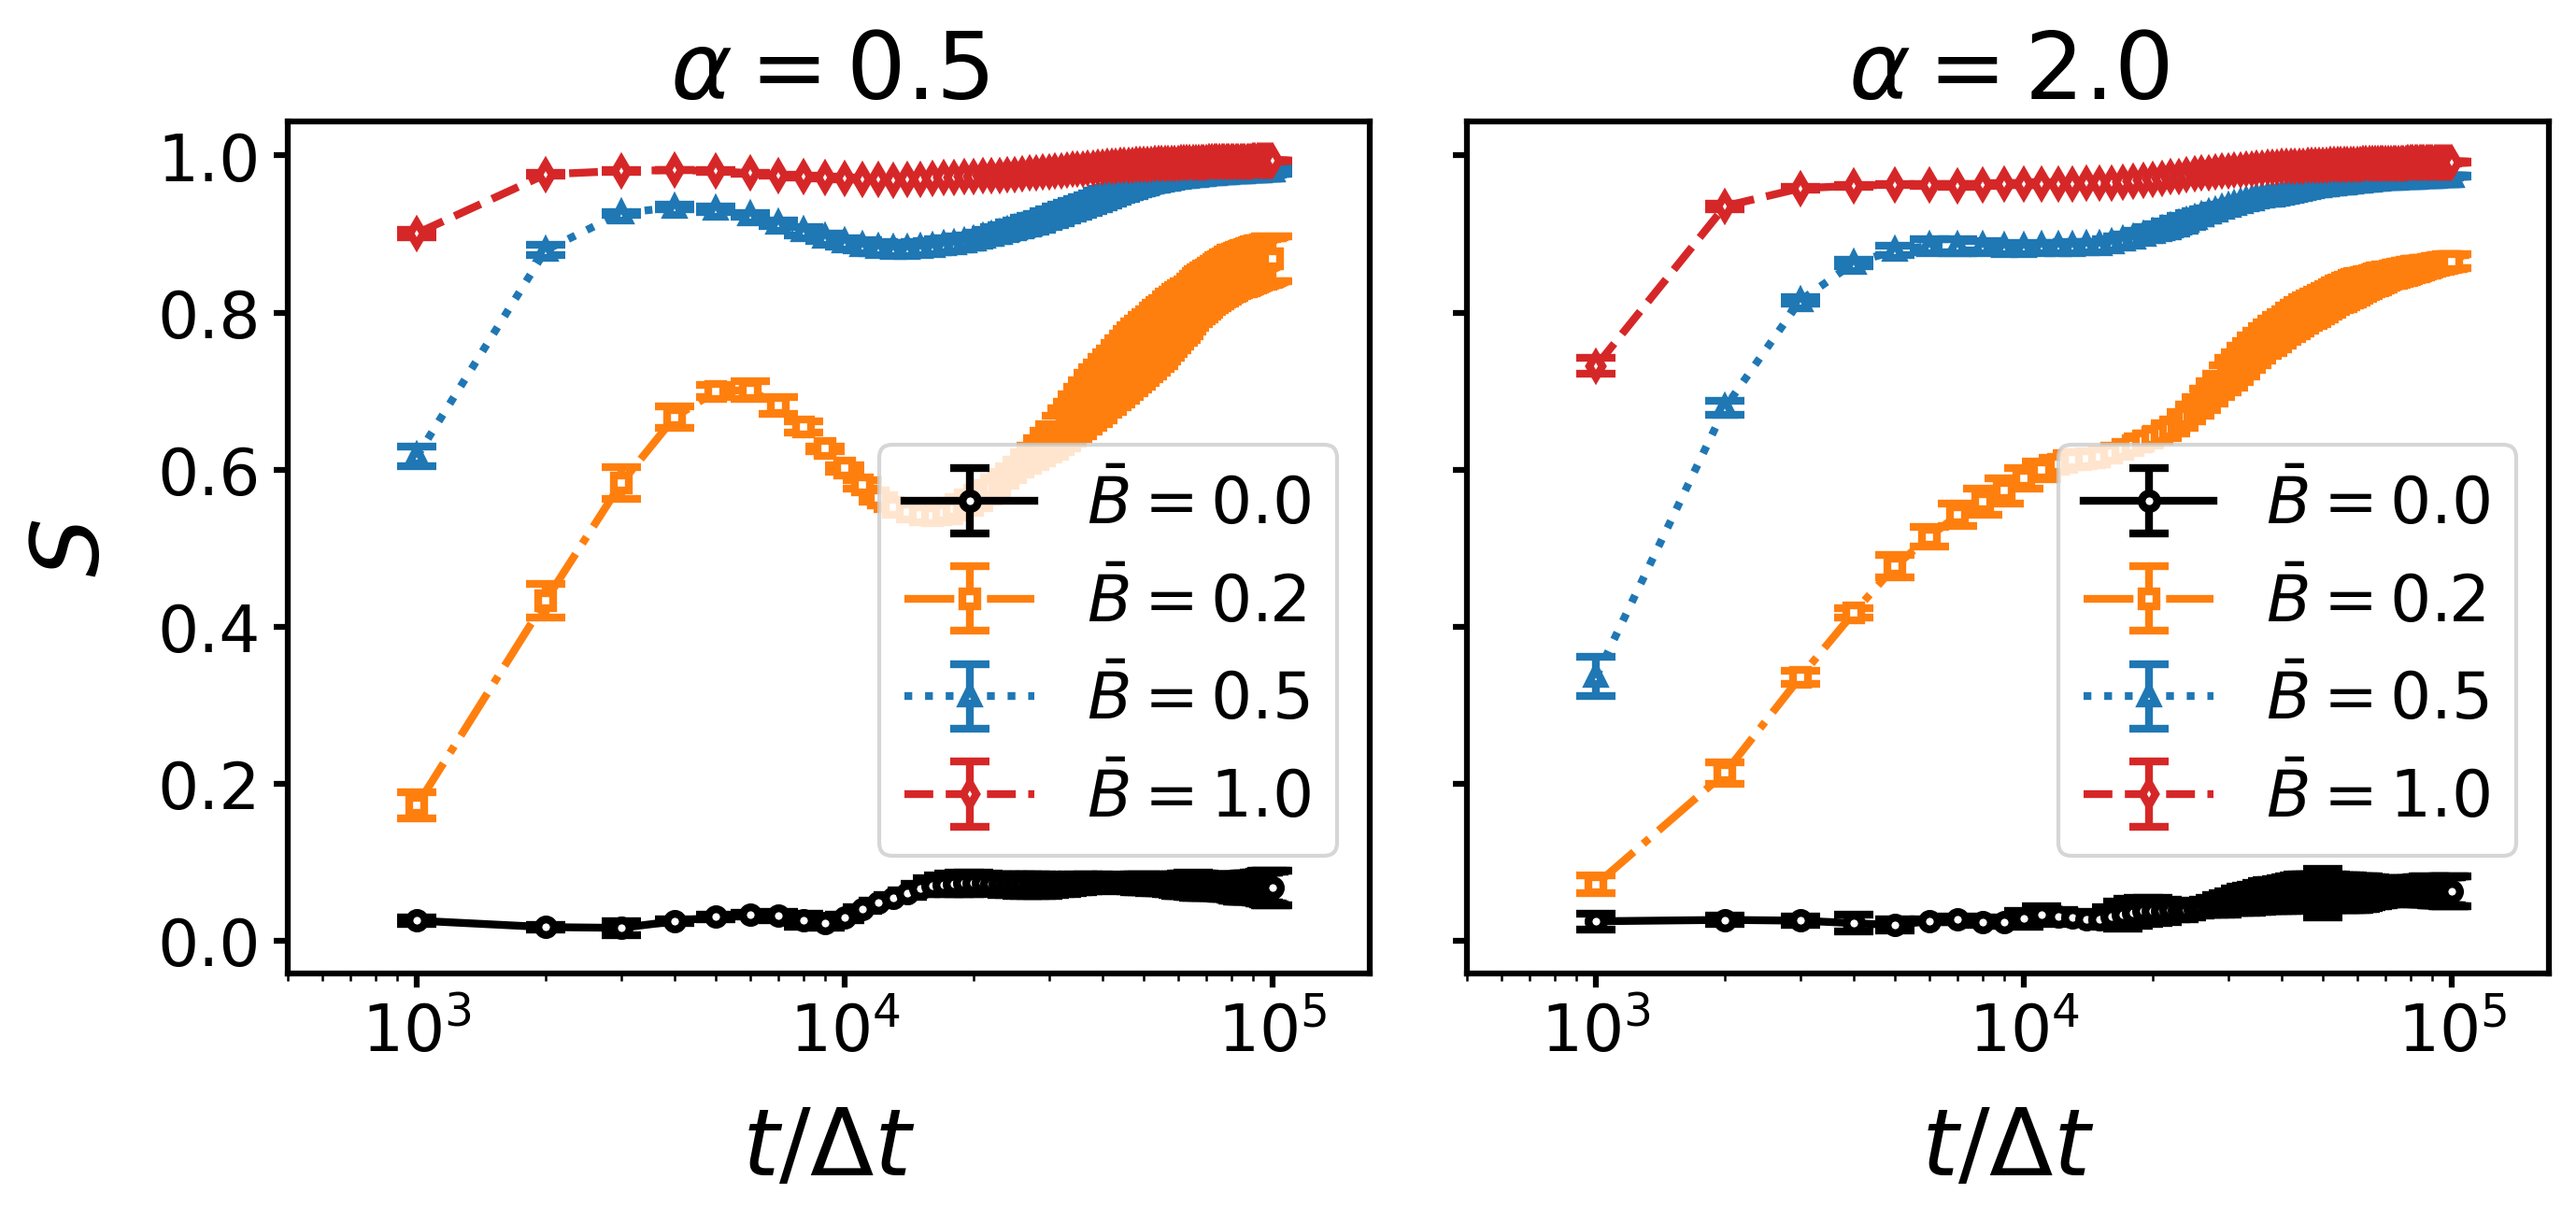
\includegraphics[width=\columnwidth]{figures/results/paper1/S-vs-t.png}
\caption{Time-dependence of the nematic order parameter $S$ of oblate ($\alpha=0.5$) and prolate ($\alpha=2$) 
        particles at different field strength $\bar{B}$. Errorbars indicate the standard deviation taken over 
        three independent simulation runs. Nematic order generally increases with applied field strength for all particle geometries. 
        The increase slows down (for prolate particles) or reverses (for oblate particles) around $10^4$ timesteps.}
\label{fig:nematic_time}
\end{figure}

To measure the particle alignment quantitatively, we computed the
nematic order tensor using the method detailed in Section \ref{section:nematic_order_parameter} 
Figure \ref{fig:nematic_time} shows the time evolution of the nematic
order parameter \(S\) for the three different particle aspect ratios
\(\alpha\) and varying magnetic field strength \(\bar{B}\). The onset of
orientational order is nearly instantaneous and increases with
increasing field strength. For magnetic flux densities
\(\bar{B}\ge0.5\), the nematic order parameter saturates at
\(S\approx 1.0\) towards the end of the simulation. For the prolate
particles (\(\alpha=2.0\)), we observe a shoulder at around
\(10^4\Delta t\) and an intermittent plateau. The occurrence of this
plateau coincides with the slowed decay of the coarsening speed in Fig.
\ref{fig:coarsening_velocity}. This change in the orientational ordering
is even more distinct for the oblate particles, where the nematic order
decays intermittently before it increases again. The intermittent decay
for oblate particles, and the plateau for prolate particles, correlate
with the delayed onset of jamming in the direction perpendicular and
parallel to the magnetic field, respectively. These observations can be
interpreted as follows: The magnetic field aligns the particles with the
direction of the magnetic field early during the simulation. Due to this
alignment, the steric constraints between particles adsorbed at the
interface are reduced which allows further coarsening of the interfacial
area. However, during coarsening, the interfaces may re-orient
themselves and cause a capillary torque on the particles that competes
with the magnetic torque. This competition intermittently perturbs the
nematic order of the particles leading to the observed decay and plateau
of the nematic order parameter. Accordingly, the decay of \(S\) is most
pronounced at the weakest magnetic field \(\bar{B}=0.2\).

To further corroborate this mechanism, we quantify the orientational
order of the interfaces. We computed the interfacial orientation tensor
%
\begin{equation}
\tens{Q}_{\text{int}} = \frac{1}{\langle \mathrm{tr}(\tens{A}) \rangle} 
\left\langle \tens{A} - \frac{1}{3} \mathrm{tr}(\tens{A}) \mathsf{1} \right\rangle ,
\end{equation}
%
where the local tensor field $\tens{A}$ is defined by
%
\begin{equation}
\tens{A} = \nabla\phi\otimes\nabla\phi .
\end{equation}
%
The largest eigenvalue of $\tens{Q}$ is taken as the
interface nematic order parameter $S_{\text{int}}$.

\begin{figure}
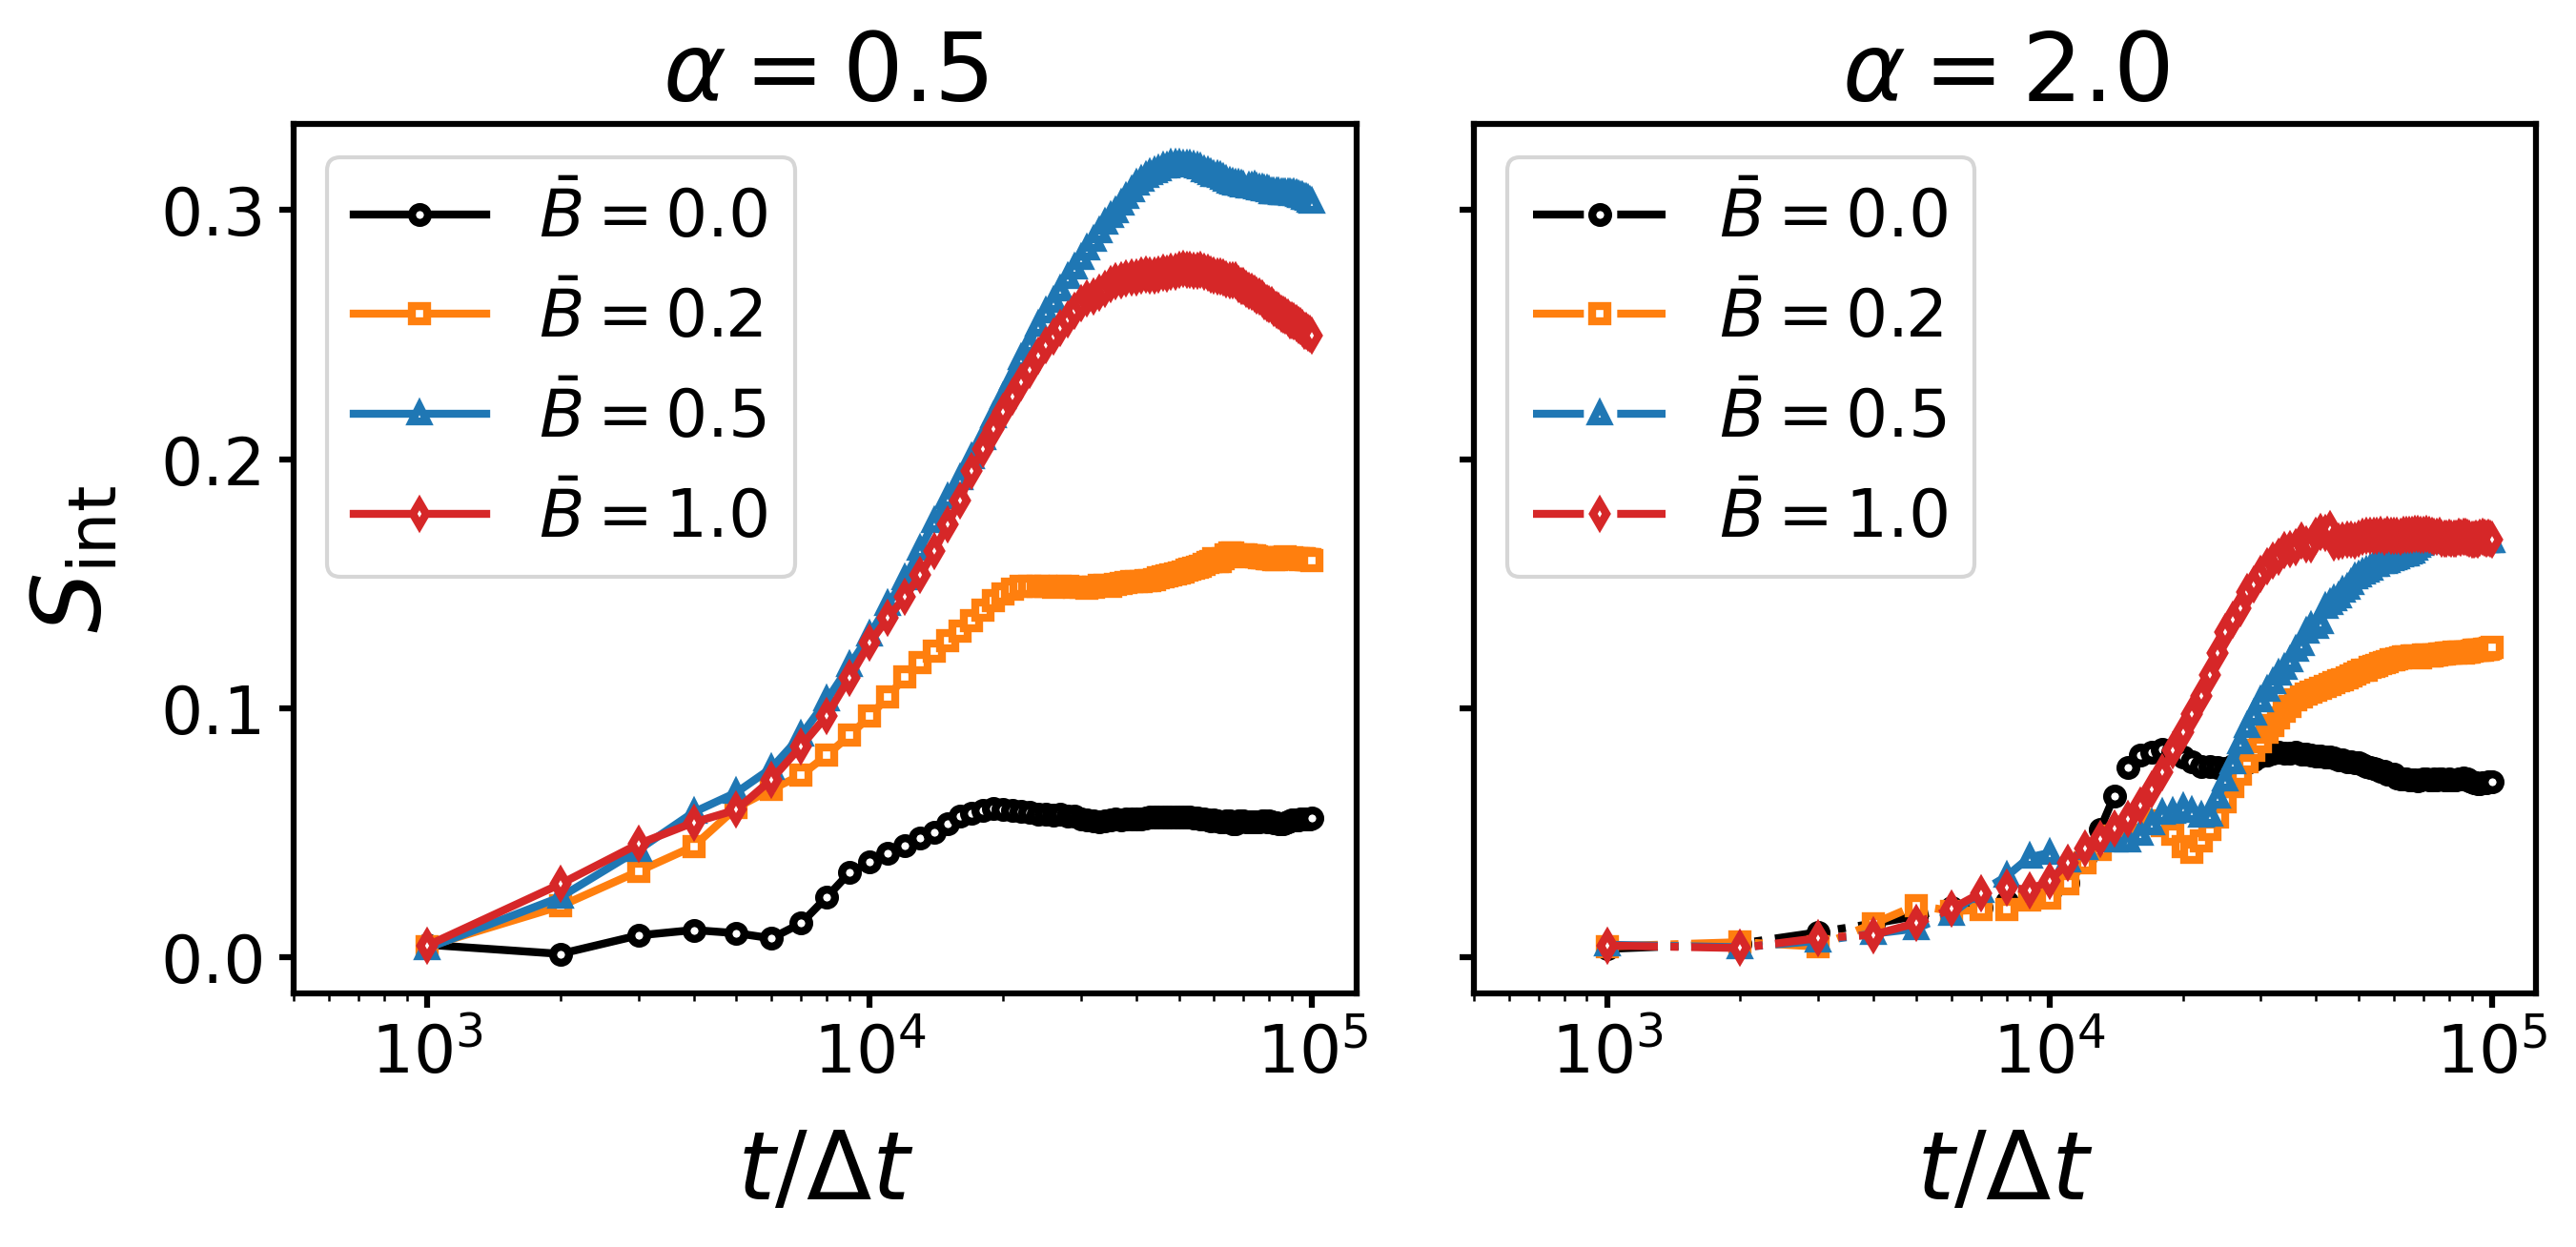
\includegraphics[width=\columnwidth]{figures/results/paper1/interface_nematic.png}
\caption{Time-dependence of the interface nematic order for oblate ($\alpha=0.5$) and prolate ($\alpha=2$) particles at different magnetic field strength $\bar{B}$. The interface alignment tends to increase with increasing field strength. The rate of increase becomes larger around $10^4$ timesteps, indicating the alignment of the interfaces due to capillary interactions with the particles.}
\label{fig:interface_nematic}
\end{figure}

The results for the interface nematic order parameter $S_{\text{int}}$
are shown in Figure \ref{fig:interface_nematic}. The nematic interface
alignment increases over time and the rate of increase appears to be
higher for larger magnetic field strength $\bar{B}$. In all cases, the
final value of $S_{\text{int}}$ is below 0.5 indicating that the
tortuous structure of the interface is maintained in the presence of
magnetic fields. This confirms that the re-orientation of the particles
does not disrupt the bijel structure but leads to partial alignment of
the interfaces without changing the general topology of the bicontinuous
morphology.

When the particles rotate, the interface exerts a capillary torque on
the particles due to the surface tension and the contact angle. If the
magnetic torque exceeds the interfacial forces, the particles can
potentially overcome the capillary torque and rotate out of the
interface. For prolate particles (\(\alpha=2\)) adsorbed at flat
interfaces, Davies et al. have shown that a transition between the
energetically preferred ``flat'' orientation and a tilted orientation
occurs at a critical field strength of approximately \(\bar{B}=0.2\)
\cite{bresme_orientational_2007,davies_interface_2014,newton_influence_2014}.
In the case of bijels, however, the percolating interfaces are tortuous
and thus more mobile. We therefore posit that, rather than tilting out
of the interface, rotating particles can ``pull'' the interface along
and thereby align the liquid domains. For anisotropic particles, we
expect that the interfaces align along the larger cross-section of the
particles, i.e., perpendicular to the symmetry axis of oblate particles
and parallel to the symmetry axis of prolate particles. The data for the
anisotropic domain size and tortuosity above is consistent with this
assumption. To ascertain that the particles remain indeed in their
energetically preferred orientation with respect to the interface, we
analyzed the angle between the symmetry axis of the particles and the
interface normal calculated using the technique defined in Section 
\ref{section:interface_angle}. Figure \ref{fig:psi_time} shows the time-dependence of the average angle
\(\psi\) between the particle dipole axis and the nearest interface normal.

\begin{figure}
\centering
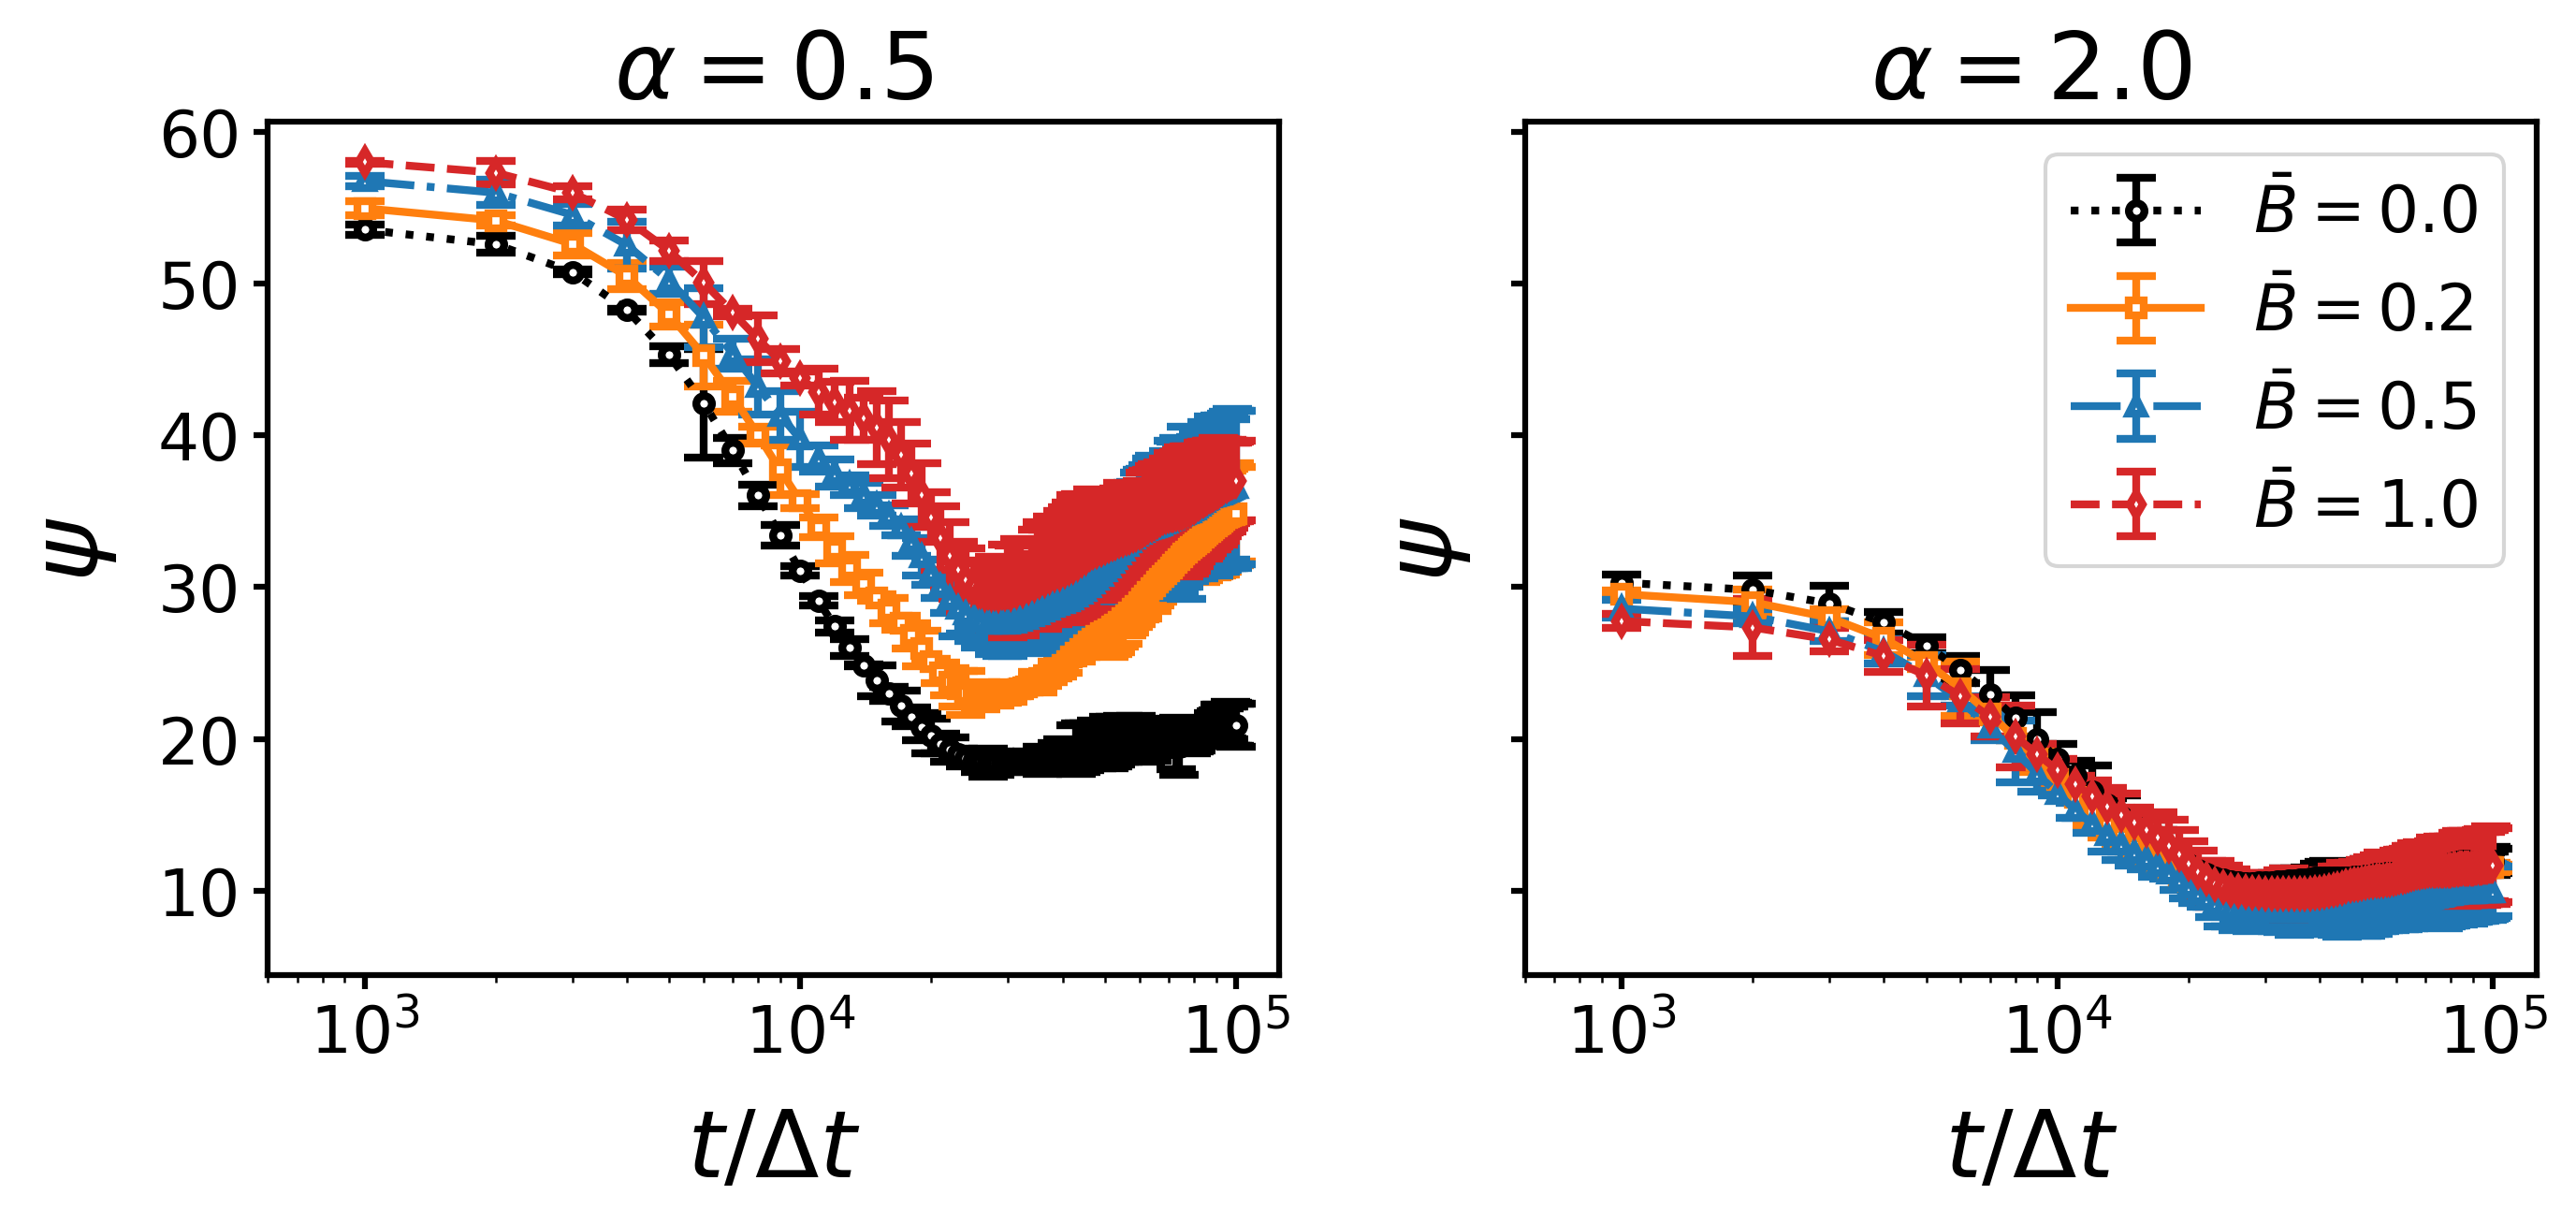
\includegraphics[width=\columnwidth]{figures/results/paper1/psi-vs-t.png}
\caption{Time-dependence of the average angle $\psi$ between the particle axis and the 
        interface normal for oblate ($\alpha=0.5$) and prolate ($\alpha=2$) particles at different 
        magnetic field strength $\bar{B}$. Errorbars indicate the standard deviation taken over three 
        independent simulation runs. The angle between between the particles and the interface normal generally 
        approaches the energetically preferred value ($0^\circ$ for oblate particls, $90^\circ$ for prolate particles).
        The average angle changes most rapidly around $10^4$ timesteps.}
\label{fig:psi_time}
\end{figure}

For both types of anisotropic particles, the average angle between the
particle dipole and the interface normal is initially around
\(\psi\approx60^\circ\). As the spinodal interface sweeps through the
system, particles attach to the interface and alignment due to the
capillary torque sets in. For oblate particles, the dipole axis aligns
with the interface normal as indicated by the decay of \(\psi\) towards
zero. For prolate particles, the preferential alignment of the dipole
axis is parallel to the interface and hence \(\psi\) increases towards
\(90^\circ\). The main variation of \(\psi\) occur in a time interval
around \(10^4\Delta t\) which coincides with the distinct features of
the coarsening speed and the particle nematic order observed above. The
results thus substantiate the proposed mechanism of particle
re-orientation in the magnetic field and the concomitant local alignment
of the interface. Once the particles start jamming, the shrinking
interfacial area forces some particles out of their preferred alignment
with the interface, leading to an increase of \(\psi\) for oblate
particles and a decrease of \(\psi\) for prolate particles. Figure
\ref{fig:psi_time} suggests that the forced tilting is more pronounced
for oblate particles than for prolate particles. Due to the larger
aspect ratio, the tilting of prolate particles relative to the interface
induces deformations that appear to cause a larger capillary torque than
the tilting of oblate particles. %For oblate particles, the liquid-solid
%contact line is on average further away from the particle center than
%for prolate particles, hence the lever effect of oblate particles is
%weaker and allows larger tilting relative to the the preferred alignment
%with the interface.
Hence the prolate particles remain mostly aligned with the interface
even in the stronger applied magnetic fields.

Information on the average ordering of the particles towards a
direction can be characterized using the nematic order parameter.
\cite{veerman_phase_1992, gunther_timescales_2014} However, we would
like to understand the local ordering of the particles over time. We
utilize the 6 fold Steinhardt order parameter Q6.
\cite{steinhardt_bond-orientational_1983, lechner_accurate_2008, mickel_shortcomings_2013} 
This parameter has been used extensively to characterize nucleation
rates, glass transitions of colloidal systems and crystal structure
transitions of ceramics and colloidal crystals.
\cite{vagberg_glassiness_2011, besseling_three-dimensional_2007, schall_structural_2007}
The original implementation has been further improved through the use an
averaged bond order parameter, adding the next nearest neighbor to the
neighbor list or utilizing voronoi cells to define the neighbor list
instead of a cutoff distance. The latter provides the more robust
implementation of the bond order parameter and is implemented in the
package Freud. \cite{ramasubramani_freud_2020} This method has been used
to characterize the jamming of discs at interfaces.
\cite{ozawa_jamming_2012} We select \(Q6\) as the parameter to calculate
due to the hexagonal ordering seen in the visualizations of the particle
monolayer. We plot the averaged bond order parameter for each timestep,
\(\langle Q6 \rangle\) calculated using a neighbor list derived from
voronoi cells below.

\begin{figure} 
    \centering 
    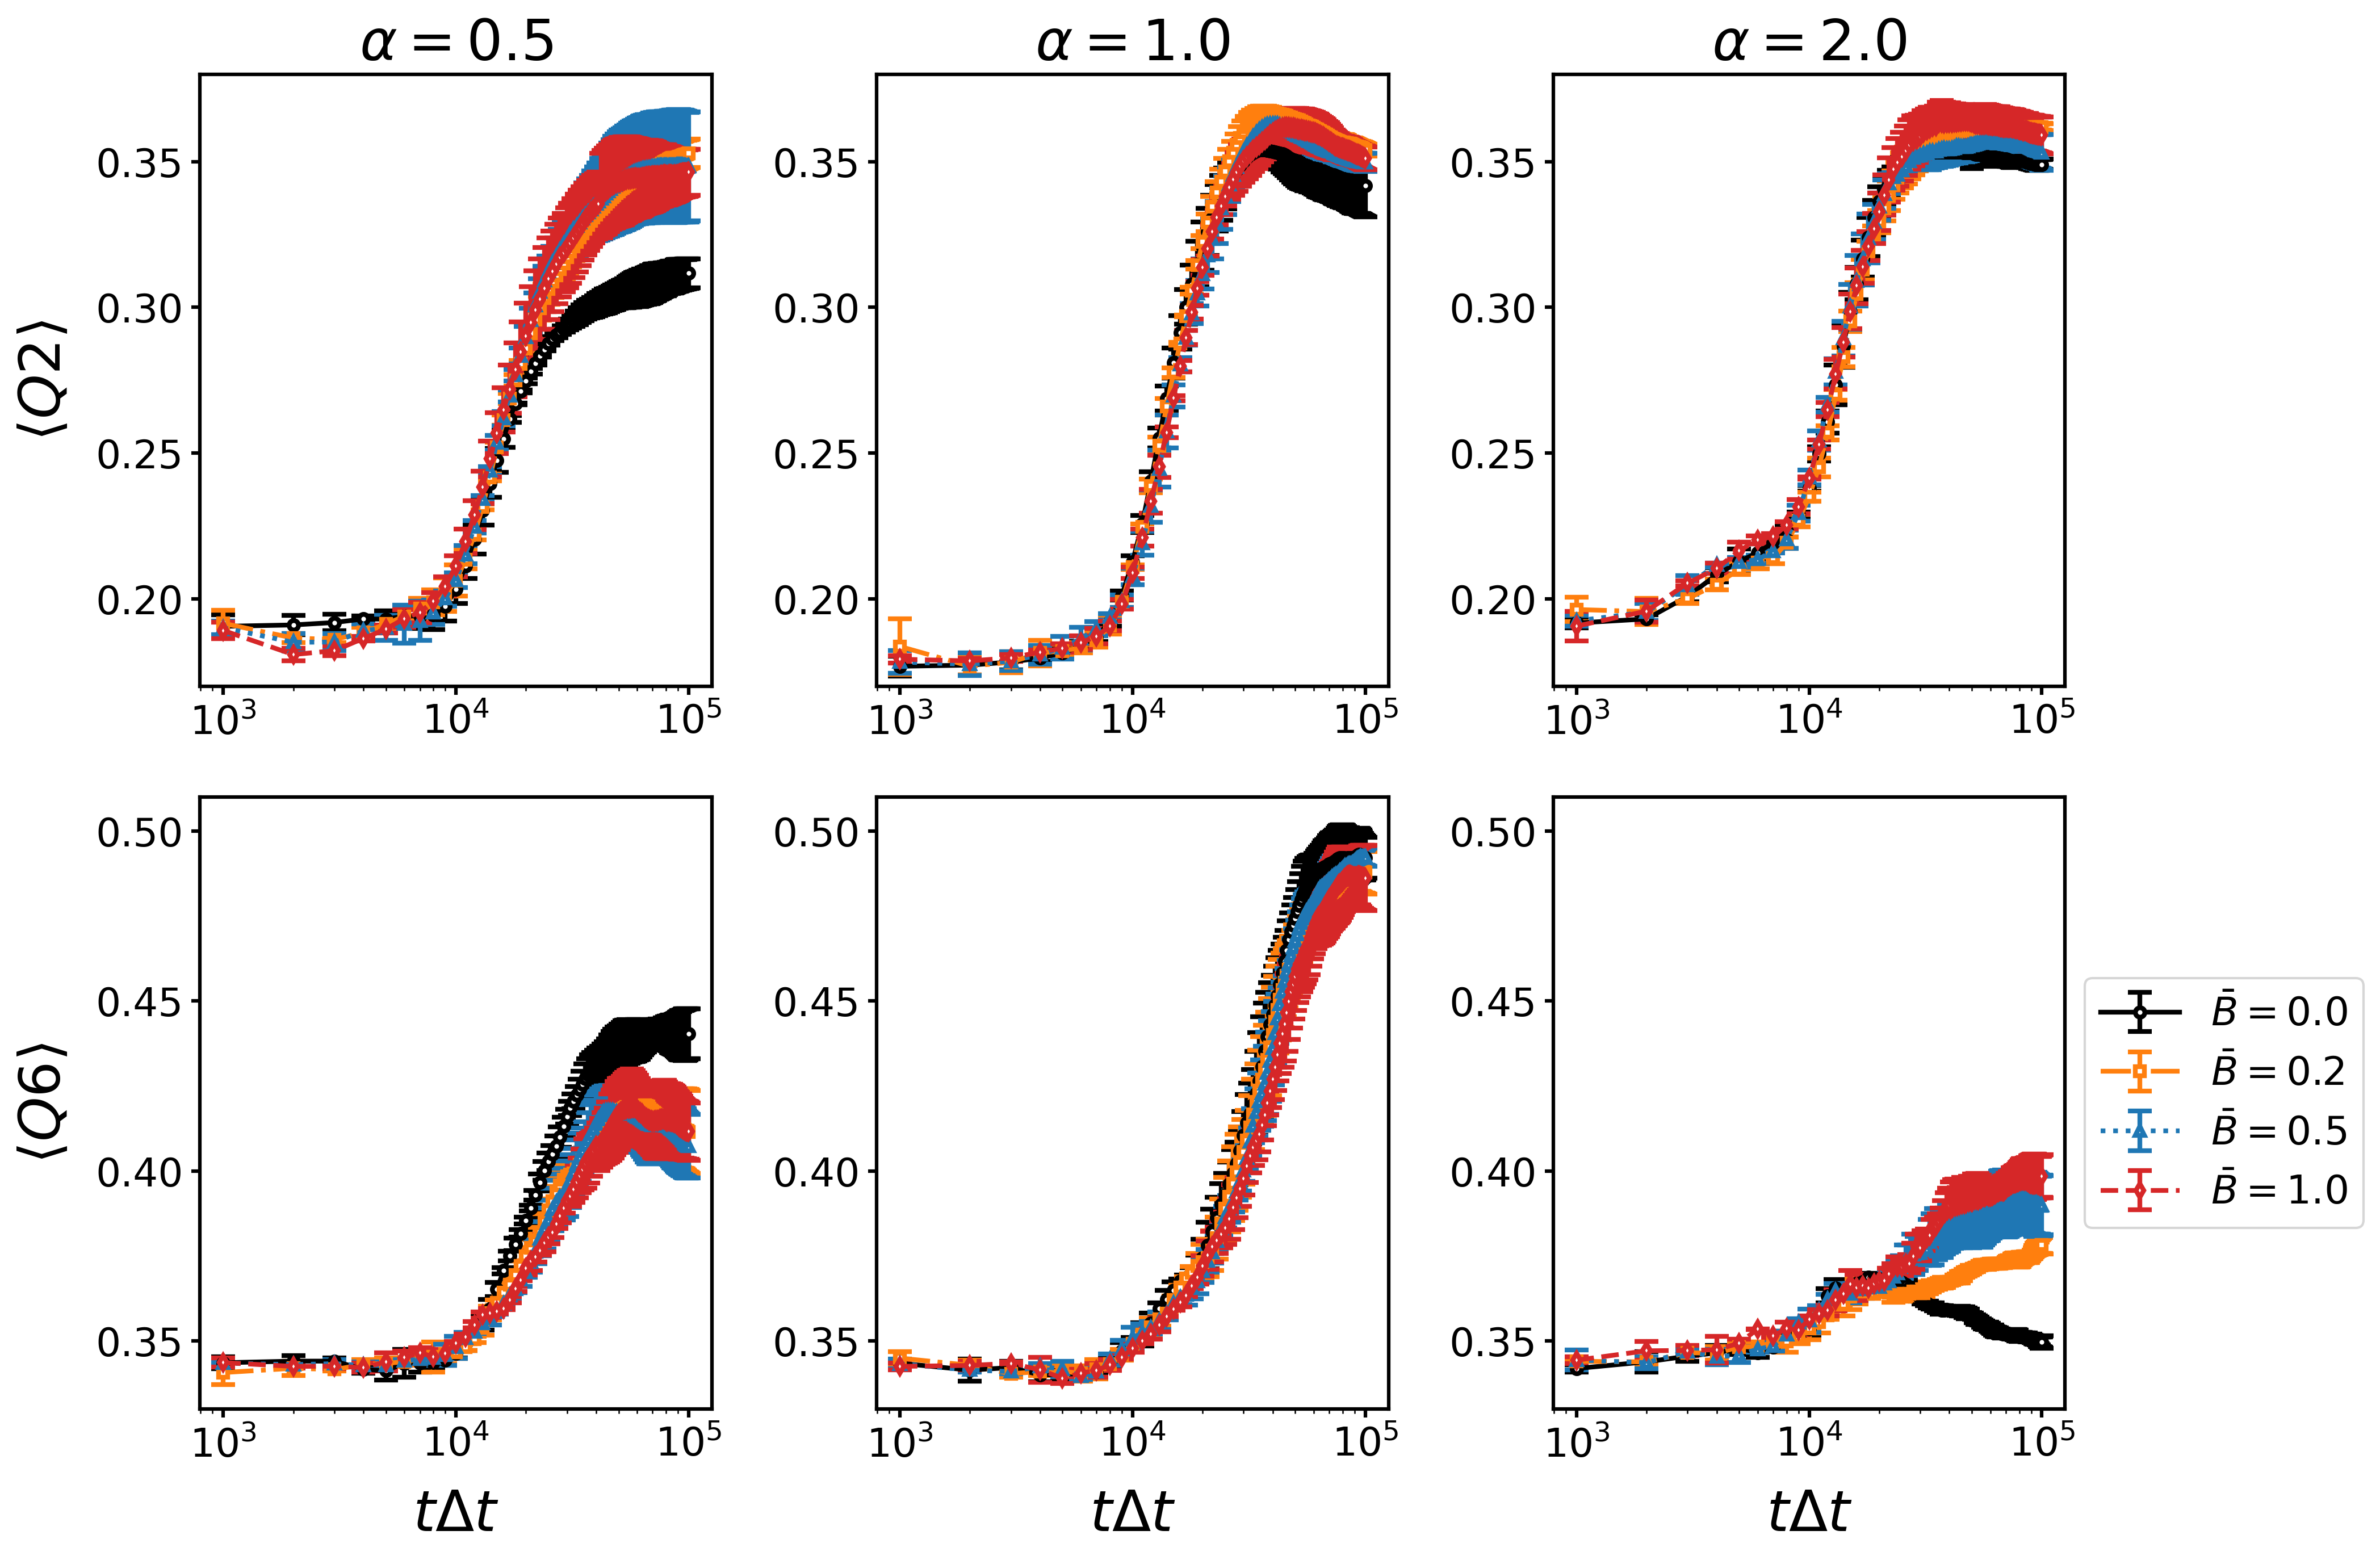
\includegraphics[width=\columnwidth]{figures/results/paper1/steinhardt_vs_coverage.png} 
    \caption{Time dependence of the mean six fold symmetry parameter, $\langle Q6 \rangle$ for bijels 
    stabilized with oblate(left), spherical(middle) and prolate(right) particles. We show that spherical 
    particles posess the hexagonal close packing structure for particles on interfaces. Ellipsoidal particles 
    however posess behavior that is magnetic field and particle aspect ratio dependent.} 
    \label{fig:Q6_coverage} 
\end{figure}

From Figure \ref{fig:Q6_coverage}, we observe that
\(\langle Q6 \rangle \approx 0.34\) for all systems before increasing.
For bijels stabilized with spherical particles, we observe that
\(\langle Q6 \rangle\) monotonically increases until
\(\langle Q6 \rangle \approx 0.485\), indicating that the spherical
particles reach a hexagonally arranged state at the interface upon
jamming. In contrast, oblate and prolate particles respectively at the
\(t = 10^5\) timesteps have values \(\langle Q6 \rangle \approx 0.44\)
and \(\langle Q6 \rangle \approx 0.35\) respectively, indicating that
the arrangement of colloids on the interface are not hexagonal close
packed. We can verify these observations in the visualizations in
Figures \ref{fig:microstructure_viz}

We observe a magnetic field dependent increase in \(\langle Q6 \rangle\)
for prolate particles to \(\langle Q6 \rangle \approx 0.4\) and decrease
for oblate particles to \(\langle Q6 \rangle \approx 0.42\). As the
magnetic field strength is increased, we observed the interface
possessed a more negative gaussian curvature. Previous work by Cavallaro
et al.~demonstrated that surfaces with large gaussian curvature
gradients can be utilized to control particle self assembly at
interfaces owing to the excess interfacial energy induced by the
curvature gradient. \cite{cavallaro_curvature-driven_2011} Spherical
particles have monopolar effects which for the colloid sizes we are
modelling are negligible. Previous literature has also ascertained
aspect ratio dependent self-assembly of ellipsoids. We attribute the
changes in the local ordering to be due to aspect ratio dependent self
assembly, amplified by the greater curvature gradient present upon
application of a magnetic field. Next, we analyze how these local
toplogical changes affect the microstructure of the bijel by analyzing
the width of the domains in the bijel.

As hypothesized above, the alignment of the particle dipole axis with
the magnetic field reduces the steric constraints within the interface.
To corroborate this idea, we analyzed the radial distribution function
(RDF) of the particles, the calculation of which is detailed in Section
\ref{section:radial_distribution} The time-evolution of the RDFs for the three particle shapes and
varying magnetic flux density is illustrated in Figure \ref{fig:rdf}.

\begin{figure*}
\centering
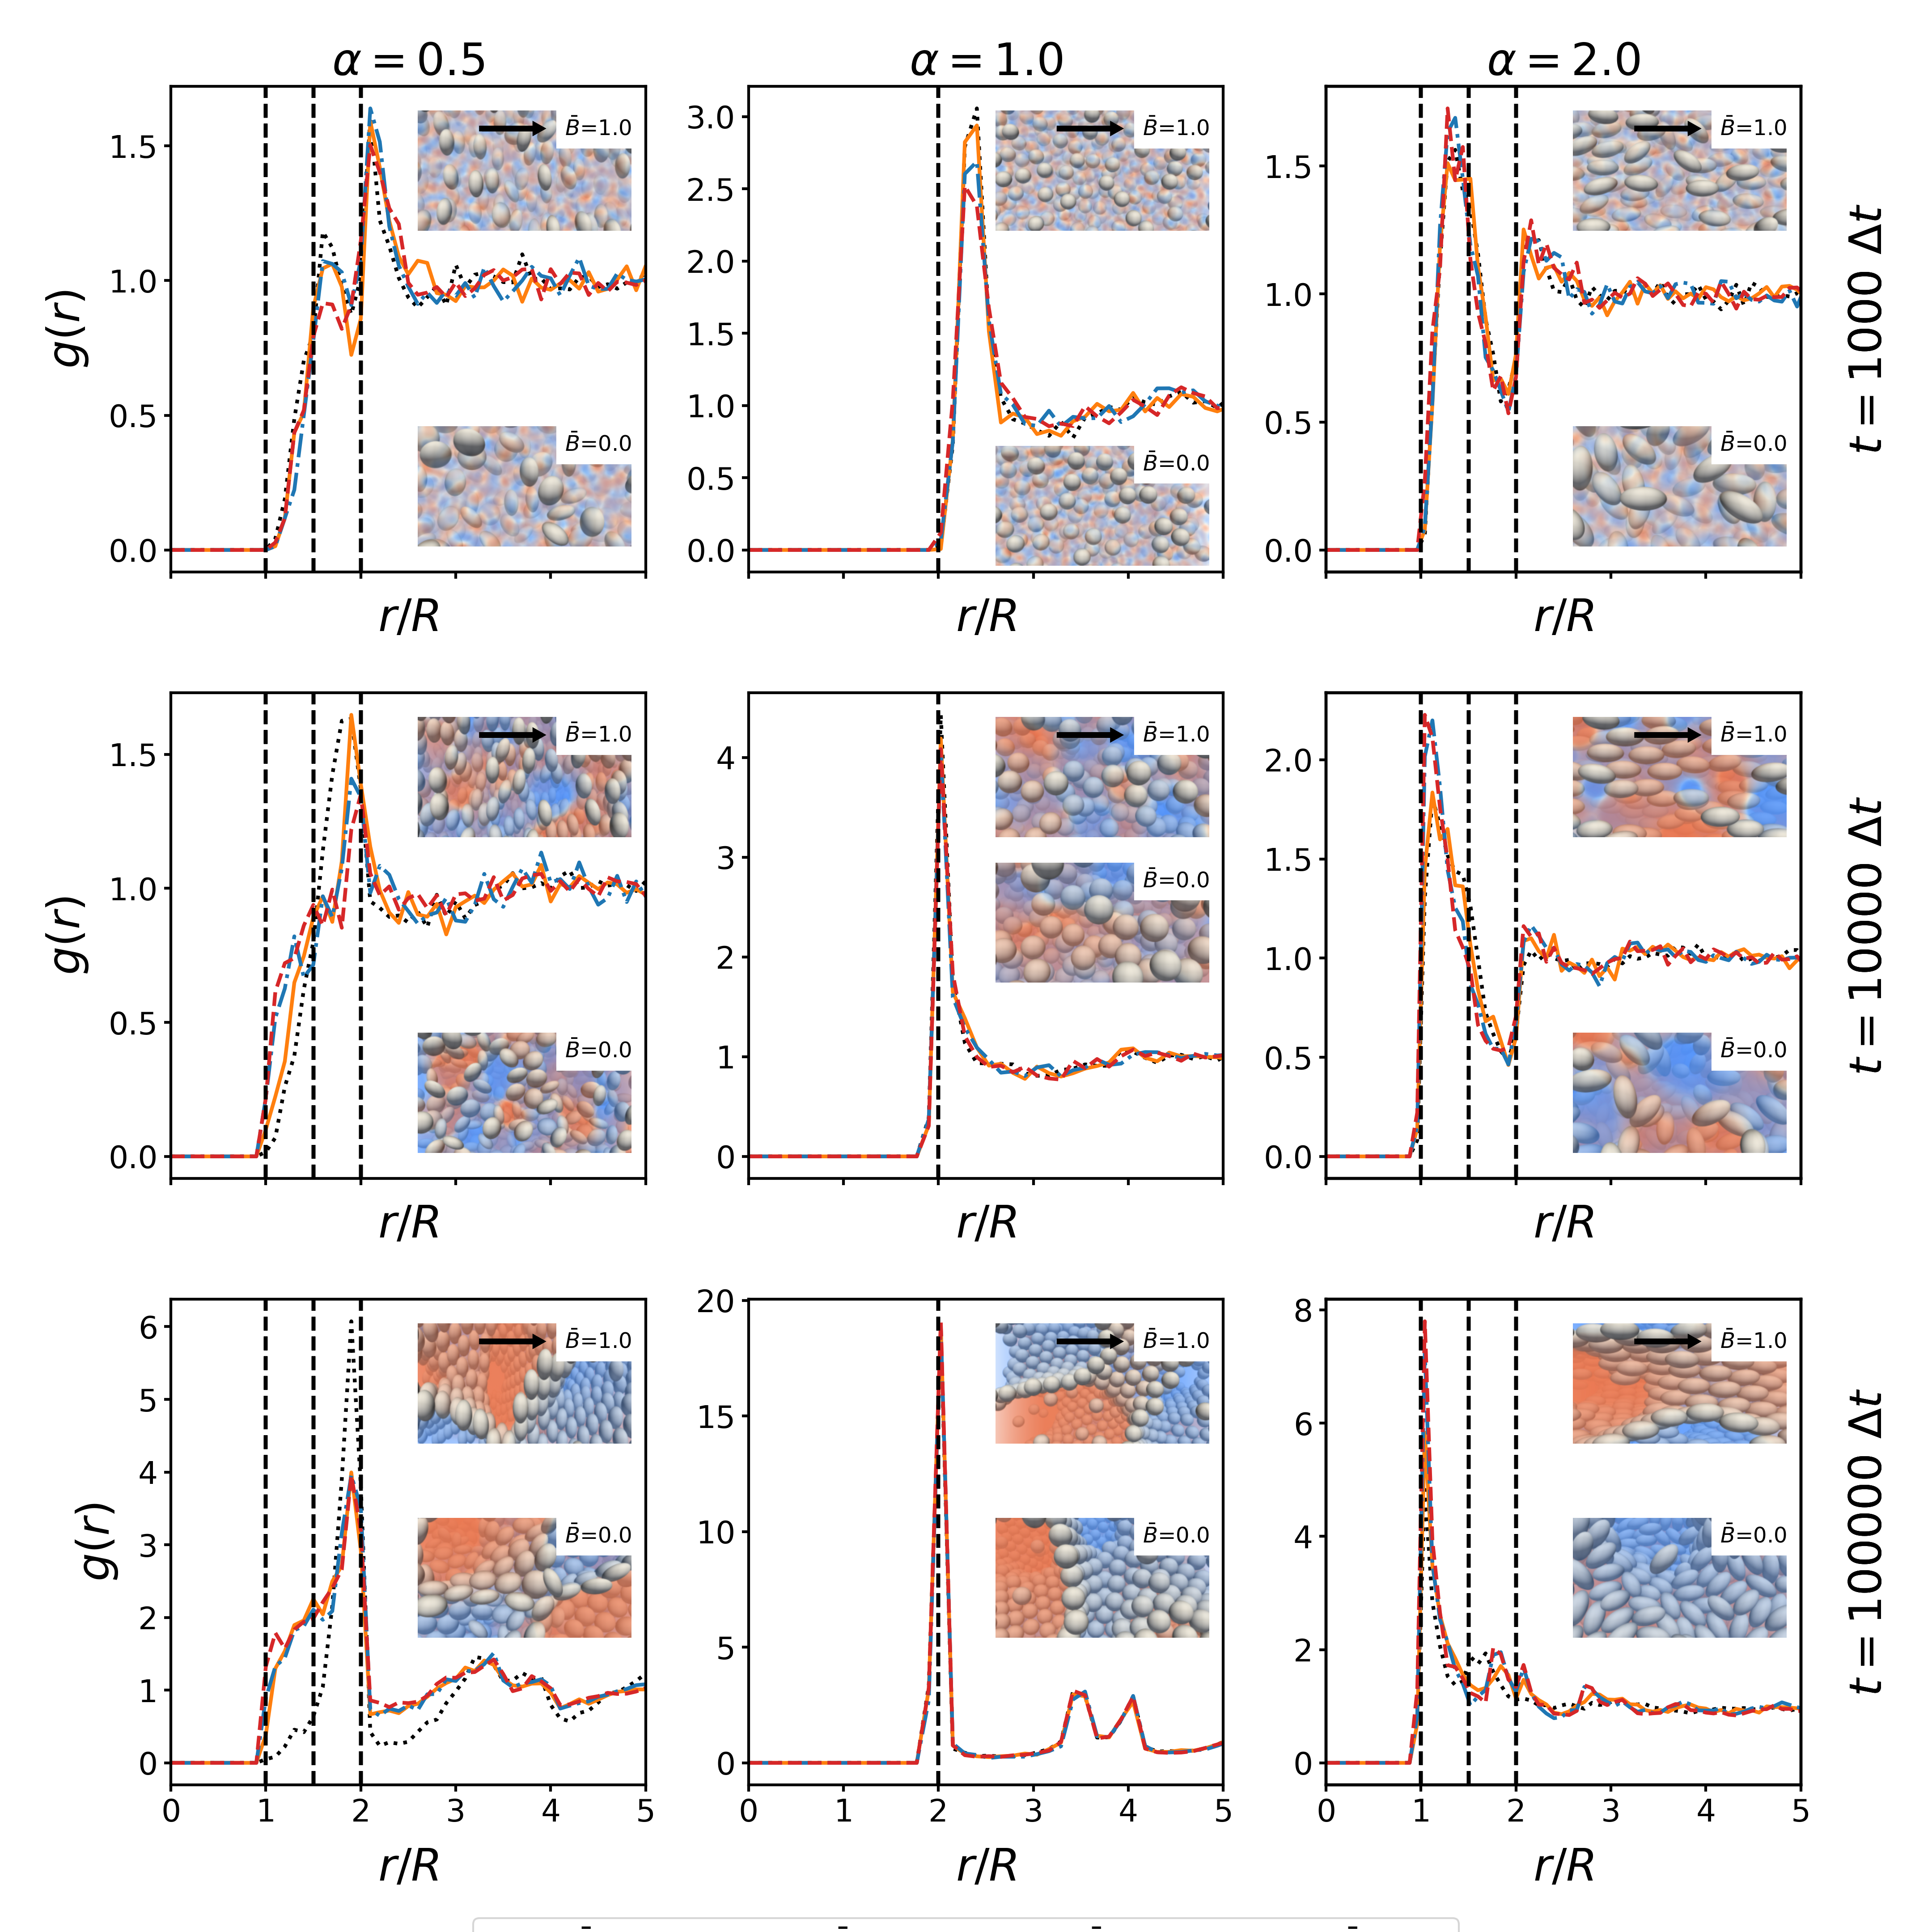
\includegraphics[width=\textwidth]{figures/results/paper1/rdf_compare_time.png}
\caption{Time-evolution of the radial distribution function $g(r)$ of the particles at different magnetic 
        field strength $\bar{B}$. The radial distribution function is shown at $10^3$, $10^4$, and $10^5$ timesteps. 
        The distance $r$ is normalized by the radius $R=\max(R_\parallel,R_\perp)$ of the larger particle axis. The peaks 
        illustrate the packing of particles in the interface. Dashed lines indicate the side-by-side, tip-to-tip, 
        and side-to-tip configuration of particle pairs. For spherical particles, the three values are identical. 
        The insets show snapshots of the particle arrangement with and without magnetic field at the respective timesteps. 
        The direction of the magnetic field is indicated by arrows.}
\label{fig:rdf}
\end{figure*}

The radial distribution function is shown at time steps
\(t=1000\Delta t,\ 10000\Delta t,\ 100000\Delta t\). For ellipsoidal
particles, the characteristic distances between particles in contact are
\(2R_{\parallel}\), \(2R_{\perp}\), and \(R_{\parallel} + R_{\perp}\).
These distances are marked by dashed lines in Fig. \ref{fig:rdf}. We
observe that the largest peak of the RDF coincides with the distance
\(2R_\perp\) for both oblate and spherical particles, indicating that
oblate particles tend to be in contact at their circumference while
prolate particles preferentially align side-by-side. These arrangements
lead to closer packing of particles in the interface. The peaks are less
pronounced in the early stage of the simulations, where the particles
are more randomly oriented. Notably, there is a dip in the RDF of
prolate particles at \(2R_\parallel\) indicating that initially the
tip-to-tip configuration occurs more rarely. The growth of the peak
height over time shows that the magnetic fields promote this alignment
compared to the case without magnetic field. For oblate particles, a
shoulder develops around \(R_\parallel+R_\perp\), indicating that some
particles tilt out of the interface to reduce the covered interfacial
area. For prolate particles, the dip at \(2R_\parallel\) disappears over
time, indicating that more particles align tip-to-tip. This is
consistent with alignment of prolate particles with respect to the
magnetic field, which facilitates closer packing along both axes of the
particles. It further suggests that particles arrange in layers, which can also be observed in the snapshot in Fig.
\ref{fig:packing_viz}. Together with the analysis of nematic order
above, these results substantiate the proposed mechanisms that influence
the formation of bijels with anisotropic particles in magnetic fields:
The magnetic field aligns the particle dipole axis in the field
direction, and the particle re-orientation couples to interface
alignment due to the capillary interactions. The alignment of particles
reduces the steric constraints within the interface, which allows the
interface to shrink further and facilitates domain coarsening. In terms
of the time-evolution, the rotation of particles due to the magnetic
field occurs during the initial stages of the simulation, followed by
the local re-alignment of interfaces due to capillary interactions. In
the case of prolate particles, we observed the shrinking interface can
force particles to tilt out of their preferential alignment to facilitate
closer packing. Generally, our results show that when bijels stabilized
by anisotropic magnetic particles form under the influence of a magnetic
field, the domain size and tortuosity become anisotropic. Additionally,
we observe that the particle packing in the interface becomes more
ordered due to the alignment effects.

\section{Conclusions}

In this work, we studied the effect of applied magnetic fields on the
formation of bijels stabilized by magnetic ellipsoidal particles. We
considered oblate, spherical, and prolate particles with a permanent
magnetic dipole moment suspended in a symmetric binary liquid. We found
that, while the overall formation of a bijel is not disrupted by
magnetic interactions, bijels stabilized by oblate or prolate ellipsoids
exhibit anisotropic domain size and an anisotropic tortuosity. For
oblate particles, the domain size increases in the direction
perpendicular to the magnetic field while the tortuosity increases in
the parallel direction. Conversely, for prolate particles, the domain
size increases in the direction parallel to the magnetic field while the
tortuosity increases in the perpendicular direction. Compared with
bijels formed in the absence of a magnetic field, we observed changes in
domain size up to \(30\%\) for non-spherical particles. This effect can
be explained by the re-orientation of the particle dipole axis with the
magnetic field, which in turn re-aligns the interfaces in the direction
of the longer axis of the particles. We further corroborated this
mechanisms by analyzing the coarsening speed and the nematic order of
the particles and the interfaces. We found that jamming of particles is
delayed in the direction of the longer ellipsoidal axis leading to
enhanced coarsening in this direction. The timescale of the delayed
jamming coincides with a slow-down of the orientational ordering of the
particles whereas the alignment of the interfaces increases. We also
found that the angle between the particle dipole axis and the interface
normal changes at this stage. Additionally, we analyzed the radial
distribution function of the particles and found that prolate particles
tend to align side by side, while the oblate particles exhibit a less
regular arrangement. Based on these findings, we propose that bijel
formation in magnetic fields is governed by two coupled effects: During
the initial stage, the magnetic torque rotates the particles to align
the magnetic dipole moment with the field, and the orientational order
of the particles facilitates further coarsening. As coarsening proceeds,
the capillary interactions cause the interfaces to align with the longer
particle axis. The shrinking interface compresses the particles into
ordered arrangements. When jamming sets in, some particles can be forced
to tilt out of the interface and this effect is more prominent for
oblate particles.

Our results demonstrate the effects of magnetic fields on the structural
properties of bijels stabilized by ellipsoidal magnetic particles. This
control is desirable in applications where the domain size and
tortuosity affect the transport properties. For example, reduced
tortuosity can increase the diffusive permeability of bone-like
materials \cite{prakoso2023tortuosity}. Similarly, low tortuosity
in lithium electrodes facilitates homogeneous ion transport and
uniform lithium deposition, leading to enhanced cyclability of
batteries\cite{chen_tortuosity_2020, ebner_tortuosity_2014}. Whereas we
have considered one particular regime of spinodal decomposition, the
viscosity and surface tension of the liquids offer additional parameters
that could be leveraged to tune the bijel formation. Moreover, the
particle volume fraction is another parameter that is known to affect
the formation of particle-stabilized emulsions
\cite{jansen_bijels_2011,hijnen_bijels_2015}. With respect to possible
experimental realizations of our simulations, we should emphasize that
we have generally considered micron-size particles and have neglected
thermal fluctuations. At the nanoscale, thermal fluctuations may in
principle play a role, however, Reeves et
al.~\cite{reeves_particle-size_2015} have shown that nanoparticles
benefit from smaller driving forces towards disruptive curvature and
actually lead to more robust bijel formation. Nevertheless, the
stability of magnetically-responsive bijels is a relevant question for
applications that involve shear flows such as crossflow reactors
\cite{khan_nanostructured_2022}. Aside from particle-size and shape
effects, direct interactions between particles are a possible avenue
to tune the formation of particle-stabilized emulsions gels, as the
recent discovery of bicontinuous intraphase jammed emulsion gels
(bipjels) illustrates \cite{kinkead_bicontinuous_2019}. Another
interesting observation arising from our simulations is that the
packing order of particles in the interface appears to increase when
bijels form under the influence of a magnetic field. While such
interfacial ordering effects have been studied on planar interfaces
\cite{toor_self-assembly_2016,shi_nanoparticle_2018,kim_dynamic_2022},
they have hitherto not been reported for particle-stabilized emulsion
gels. It would be interesting to examine the implications of this
ordering on the optical and transport properties of jammed emulsion
gels. In conclusion, our simulations provide relevant insights into the
formation of magnetic particle-stabilized bijels in the presence of
external magnetic fields, and they demonstrate the potential of magnetic
particles for fabrication of emulsion systems with tunable and
anisotropic particle packing and domain structure.